% Options for packages loaded elsewhere
% Options for packages loaded elsewhere
\PassOptionsToPackage{unicode}{hyperref}
\PassOptionsToPackage{hyphens}{url}
\PassOptionsToPackage{dvipsnames,svgnames,x11names}{xcolor}
%
\documentclass[
  11pt,
  a4paper,
]{article}
\usepackage{xcolor}
\usepackage[lmargin=2cm,rmargin=2cm,tmargin=2cm,bmargin=2cm]{geometry}
\usepackage{amsmath,amssymb}
\setcounter{secnumdepth}{5}
\usepackage{iftex}
\ifPDFTeX
  \usepackage[T1]{fontenc}
  \usepackage[utf8]{inputenc}
  \usepackage{textcomp} % provide euro and other symbols
\else % if luatex or xetex
  \usepackage{unicode-math} % this also loads fontspec
  \defaultfontfeatures{Scale=MatchLowercase}
  \defaultfontfeatures[\rmfamily]{Ligatures=TeX,Scale=1}
\fi
\usepackage{lmodern}
\ifPDFTeX\else
  % xetex/luatex font selection
\fi
% Use upquote if available, for straight quotes in verbatim environments
\IfFileExists{upquote.sty}{\usepackage{upquote}}{}
\IfFileExists{microtype.sty}{% use microtype if available
  \usepackage[]{microtype}
  \UseMicrotypeSet[protrusion]{basicmath} % disable protrusion for tt fonts
}{}
\makeatletter
\@ifundefined{KOMAClassName}{% if non-KOMA class
  \IfFileExists{parskip.sty}{%
    \usepackage{parskip}
  }{% else
    \setlength{\parindent}{0pt}
    \setlength{\parskip}{6pt plus 2pt minus 1pt}}
}{% if KOMA class
  \KOMAoptions{parskip=half}}
\makeatother
% Make \paragraph and \subparagraph free-standing
\makeatletter
\ifx\paragraph\undefined\else
  \let\oldparagraph\paragraph
  \renewcommand{\paragraph}{
    \@ifstar
      \xxxParagraphStar
      \xxxParagraphNoStar
  }
  \newcommand{\xxxParagraphStar}[1]{\oldparagraph*{#1}\mbox{}}
  \newcommand{\xxxParagraphNoStar}[1]{\oldparagraph{#1}\mbox{}}
\fi
\ifx\subparagraph\undefined\else
  \let\oldsubparagraph\subparagraph
  \renewcommand{\subparagraph}{
    \@ifstar
      \xxxSubParagraphStar
      \xxxSubParagraphNoStar
  }
  \newcommand{\xxxSubParagraphStar}[1]{\oldsubparagraph*{#1}\mbox{}}
  \newcommand{\xxxSubParagraphNoStar}[1]{\oldsubparagraph{#1}\mbox{}}
\fi
\makeatother

\usepackage{color}
\usepackage{fancyvrb}
\newcommand{\VerbBar}{|}
\newcommand{\VERB}{\Verb[commandchars=\\\{\}]}
\DefineVerbatimEnvironment{Highlighting}{Verbatim}{commandchars=\\\{\}}
% Add ',fontsize=\small' for more characters per line
\usepackage{framed}
\definecolor{shadecolor}{RGB}{241,243,245}
\newenvironment{Shaded}{\begin{snugshade}}{\end{snugshade}}
\newcommand{\AlertTok}[1]{\textcolor[rgb]{0.68,0.00,0.00}{#1}}
\newcommand{\AnnotationTok}[1]{\textcolor[rgb]{0.37,0.37,0.37}{#1}}
\newcommand{\AttributeTok}[1]{\textcolor[rgb]{0.40,0.45,0.13}{#1}}
\newcommand{\BaseNTok}[1]{\textcolor[rgb]{0.68,0.00,0.00}{#1}}
\newcommand{\BuiltInTok}[1]{\textcolor[rgb]{0.00,0.23,0.31}{#1}}
\newcommand{\CharTok}[1]{\textcolor[rgb]{0.13,0.47,0.30}{#1}}
\newcommand{\CommentTok}[1]{\textcolor[rgb]{0.37,0.37,0.37}{#1}}
\newcommand{\CommentVarTok}[1]{\textcolor[rgb]{0.37,0.37,0.37}{\textit{#1}}}
\newcommand{\ConstantTok}[1]{\textcolor[rgb]{0.56,0.35,0.01}{#1}}
\newcommand{\ControlFlowTok}[1]{\textcolor[rgb]{0.00,0.23,0.31}{\textbf{#1}}}
\newcommand{\DataTypeTok}[1]{\textcolor[rgb]{0.68,0.00,0.00}{#1}}
\newcommand{\DecValTok}[1]{\textcolor[rgb]{0.68,0.00,0.00}{#1}}
\newcommand{\DocumentationTok}[1]{\textcolor[rgb]{0.37,0.37,0.37}{\textit{#1}}}
\newcommand{\ErrorTok}[1]{\textcolor[rgb]{0.68,0.00,0.00}{#1}}
\newcommand{\ExtensionTok}[1]{\textcolor[rgb]{0.00,0.23,0.31}{#1}}
\newcommand{\FloatTok}[1]{\textcolor[rgb]{0.68,0.00,0.00}{#1}}
\newcommand{\FunctionTok}[1]{\textcolor[rgb]{0.28,0.35,0.67}{#1}}
\newcommand{\ImportTok}[1]{\textcolor[rgb]{0.00,0.46,0.62}{#1}}
\newcommand{\InformationTok}[1]{\textcolor[rgb]{0.37,0.37,0.37}{#1}}
\newcommand{\KeywordTok}[1]{\textcolor[rgb]{0.00,0.23,0.31}{\textbf{#1}}}
\newcommand{\NormalTok}[1]{\textcolor[rgb]{0.00,0.23,0.31}{#1}}
\newcommand{\OperatorTok}[1]{\textcolor[rgb]{0.37,0.37,0.37}{#1}}
\newcommand{\OtherTok}[1]{\textcolor[rgb]{0.00,0.23,0.31}{#1}}
\newcommand{\PreprocessorTok}[1]{\textcolor[rgb]{0.68,0.00,0.00}{#1}}
\newcommand{\RegionMarkerTok}[1]{\textcolor[rgb]{0.00,0.23,0.31}{#1}}
\newcommand{\SpecialCharTok}[1]{\textcolor[rgb]{0.37,0.37,0.37}{#1}}
\newcommand{\SpecialStringTok}[1]{\textcolor[rgb]{0.13,0.47,0.30}{#1}}
\newcommand{\StringTok}[1]{\textcolor[rgb]{0.13,0.47,0.30}{#1}}
\newcommand{\VariableTok}[1]{\textcolor[rgb]{0.07,0.07,0.07}{#1}}
\newcommand{\VerbatimStringTok}[1]{\textcolor[rgb]{0.13,0.47,0.30}{#1}}
\newcommand{\WarningTok}[1]{\textcolor[rgb]{0.37,0.37,0.37}{\textit{#1}}}

\usepackage{longtable,booktabs,array}
\usepackage{calc} % for calculating minipage widths
% Correct order of tables after \paragraph or \subparagraph
\usepackage{etoolbox}
\makeatletter
\patchcmd\longtable{\par}{\if@noskipsec\mbox{}\fi\par}{}{}
\makeatother
% Allow footnotes in longtable head/foot
\IfFileExists{footnotehyper.sty}{\usepackage{footnotehyper}}{\usepackage{footnote}}
\makesavenoteenv{longtable}
\usepackage{graphicx}
\makeatletter
\newsavebox\pandoc@box
\newcommand*\pandocbounded[1]{% scales image to fit in text height/width
  \sbox\pandoc@box{#1}%
  \Gscale@div\@tempa{\textheight}{\dimexpr\ht\pandoc@box+\dp\pandoc@box\relax}%
  \Gscale@div\@tempb{\linewidth}{\wd\pandoc@box}%
  \ifdim\@tempb\p@<\@tempa\p@\let\@tempa\@tempb\fi% select the smaller of both
  \ifdim\@tempa\p@<\p@\scalebox{\@tempa}{\usebox\pandoc@box}%
  \else\usebox{\pandoc@box}%
  \fi%
}
% Set default figure placement to htbp
\def\fps@figure{htbp}
\makeatother





\setlength{\emergencystretch}{3em} % prevent overfull lines

\providecommand{\tightlist}{%
  \setlength{\itemsep}{0pt}\setlength{\parskip}{0pt}}



 


\usepackage{booktabs}
\usepackage{longtable}
\usepackage{array}
\usepackage{multirow}
\usepackage{float}
\usepackage{makecell}
\makeatletter
\@ifpackageloaded{caption}{}{\usepackage{caption}}
\AtBeginDocument{%
\ifdefined\contentsname
  \renewcommand*\contentsname{Table of contents}
\else
  \newcommand\contentsname{Table of contents}
\fi
\ifdefined\listfigurename
  \renewcommand*\listfigurename{List of Figures}
\else
  \newcommand\listfigurename{List of Figures}
\fi
\ifdefined\listtablename
  \renewcommand*\listtablename{List of Tables}
\else
  \newcommand\listtablename{List of Tables}
\fi
\ifdefined\figurename
  \renewcommand*\figurename{Figure}
\else
  \newcommand\figurename{Figure}
\fi
\ifdefined\tablename
  \renewcommand*\tablename{Table}
\else
  \newcommand\tablename{Table}
\fi
}
\@ifpackageloaded{float}{}{\usepackage{float}}
\floatstyle{ruled}
\@ifundefined{c@chapter}{\newfloat{codelisting}{h}{lop}}{\newfloat{codelisting}{h}{lop}[chapter]}
\floatname{codelisting}{Listing}
\newcommand*\listoflistings{\listof{codelisting}{List of Listings}}
\makeatother
\makeatletter
\makeatother
\makeatletter
\@ifpackageloaded{caption}{}{\usepackage{caption}}
\@ifpackageloaded{subcaption}{}{\usepackage{subcaption}}
\makeatother
\usepackage{bookmark}
\IfFileExists{xurl.sty}{\usepackage{xurl}}{} % add URL line breaks if available
\urlstyle{same}
\hypersetup{
  pdftitle={Why Have House Prices in Turkey Gone Up in the Last Ten Years?},
  pdfauthor={Ömer Furkan Demirci; Fatih Alper Vural},
  colorlinks=true,
  linkcolor={blue},
  filecolor={Maroon},
  citecolor={Blue},
  urlcolor={Blue},
  pdfcreator={LaTeX via pandoc}}


\title{Why Have House Prices in Turkey Gone Up in the Last Ten Years?}
\author{Ömer Furkan Demirci \and Fatih Alper Vural}
\date{2026-05-20}
\begin{document}
\maketitle

\renewcommand*\contentsname{Table of contents}
{
\hypersetup{linkcolor=}
\setcounter{tocdepth}{3}
\tableofcontents
}

\begin{Shaded}
\begin{Highlighting}[]
\FunctionTok{options}\NormalTok{(}\AttributeTok{kableExtra.latex.load\_packages =} \ConstantTok{FALSE}\NormalTok{)}
\end{Highlighting}
\end{Shaded}

\subsection*{Abstract}\label{abstract}
\addcontentsline{toc}{subsection}{Abstract}

Housing affordability has emerged as one of the most pressing
socioeconomic challenges in Türkiye over the past decade. This study
investigates the key drivers of the sharp and sustained rise in housing
prices between 2014 and 2024, drawing on four official monthly
time-series datasets obtained from the Central Bank of the Republic of
Türkiye (TCMB/EVDS): the House Price Index (HPI), housing sales
statistics, USD/EUR exchange rates, and credit card sectoral expenditure
data. Through exploratory analysis, correlation testing, regional
comparison, and multiple linear regression modelling, we find that
exchange rate depreciation and broad consumer spending inflation are the
dominant macroeconomic forces behind rising house prices, while sales
volumes display an inverse relationship with price levels --- consistent
with demand compression at high price levels. Regional heterogeneity is
substantial: İstanbul and western metropolitan areas lead price growth,
whereas interior Anatolian regions lag considerably. Our model explains
approximately 95\% of the variance in the national HPI, suggesting that
macroeconomic indicators are strong predictors of housing price
trajectories in Türkiye.

\begin{center}\rule{0.5\linewidth}{0.5pt}\end{center}

\section{Project Overview and Scope}\label{project-overview-and-scope}

We want to look into the following question for this project:\\
\strut \\
\textbf{Why have house prices in Turkey gone up in the last ten
years?}\\
\strut \\
To answer this question, we made a dataset using four monthly
time-series datasets from the Central Bank of the Republic of Türkiye's
(TCMB) Electronic Data Delivery System (EVDS). These datasets have:\\

\begin{itemize}
\item
  Housing Price Index
\item
  Sales of Houses
\item
  Exchange Rates (USD/TRY and EUR/TRY)
\item
  Credit Card Sectoral Expenditures\\
  \strut \\
\end{itemize}

We chose this topic because the cost of housing has become one of the
most important social and economic issues in Türkiye. It is important to
know what caused this rise in order to make good decisions about policy
and the economy. This problem is also a good fit for a data analytics
approach because it needs to combine multiple datasets, do
preprocessing, and look at how things change over time and in different
areas.

We want to find the main things that cause housing prices to go up.
Specifically, we want to look at:

\begin{itemize}
\item
  How exchange rates affect the price of homes
\item
  The link between changes in housing prices and demand (sales)
\item
  The function of consumption behavior (credit card expenditure) as an
  indicator of demand conditions.
\item
  Differences in how housing works in different regions
\end{itemize}

\section{Data}\label{data}

You can see Our data in R Data format below.

\href{https://github.com/emu-hacettepe-analytics/emu660-spring2026-ofdemirci/blob/e273d93492dc0a2ea56f85a472a398fe4909c2d7/Data/Project_Data.RData}{Project
Data}

\begin{Shaded}
\begin{Highlighting}[]
\NormalTok{url }\OtherTok{\textless{}{-}} \StringTok{"https://raw.githubusercontent.com/emu{-}hacettepe{-}analytics/emu660{-}spring2026{-}ofdemirci/main/Data/Project\_Data.RData"}
\FunctionTok{download.file}\NormalTok{(url, }\AttributeTok{destfile =} \StringTok{"Project\_Data.RData"}\NormalTok{, }\AttributeTok{mode =} \StringTok{"wb"}\NormalTok{)}
\FunctionTok{load}\NormalTok{(}\StringTok{"Project\_Data.RData"}\NormalTok{)}

\FunctionTok{ls}\NormalTok{()}
\end{Highlighting}
\end{Shaded}

\begin{verbatim}
[1] "Conversion_Rates"  "Expense_Quantity"  "Konut_Index_Sales"
[4] "url"              
\end{verbatim}

\subsection{Data Source}\label{data-source}

The data used in this project were obtained from the \textbf{Electronic
Data Delivery System (EVDS)} of the Central Bank of the Republic of
Türkiye (TCMB). EVDS provides official, high-frequency economic data and
is widely used for academic and professional analysis.

The project is based on four datasets:

\begin{itemize}
\item
  \textbf{House Price Index (HPI)}\\
  Monthly housing price index at national and regional levels
\item
  \textbf{House Sales Statistics}\\
  Monthly housing sales data at the provincial level
\item
  \textbf{Exchange Rates (USD, EUR)}\\
  Monthly exchange rate data
\item
  \textbf{Credit Card Sectoral Expenditures}\\
  Monthly sector-based credit card spending data
\end{itemize}

\subsection{General Information About
Data}\label{general-information-about-data}

The processed dataset consists of three main analytical tables:

\subsubsection{Exchange Rate Table}\label{exchange-rate-table}

\begin{itemize}
\item
  \textbf{Description}:\\
  This table contains the columns Year, Month, USD Conversion Rate, and
  EUR Conversion Rate. Represents monthly exchange rate movements. These
  variables are used as indicators of macroeconomic conditions and
  cost-side pressures that may affect housing prices.
\item
  In general, the exchange rate variables show a strong upward trend
  over time rather than a stable distribution.

\begin{Shaded}
\begin{Highlighting}[]
\FunctionTok{library}\NormalTok{(dplyr)}
\FunctionTok{library}\NormalTok{(ggplot2)}
\FunctionTok{library}\NormalTok{(scales)}
\NormalTok{usd\_eur }\OtherTok{\textless{}{-}}\NormalTok{ Conversion\_Rates }\SpecialCharTok{\%\textgreater{}\%}
  \FunctionTok{filter}\NormalTok{(Year }\SpecialCharTok{\textless{}} \DecValTok{2026}\NormalTok{) }\SpecialCharTok{\%\textgreater{}\%}
  \FunctionTok{mutate}\NormalTok{(}\AttributeTok{Date =} \FunctionTok{as.Date}\NormalTok{(}\FunctionTok{sprintf}\NormalTok{(}\StringTok{"\%d{-}\%02d{-}01"}\NormalTok{, Year, Month)))}

\FunctionTok{ggplot}\NormalTok{(usd\_eur, }\FunctionTok{aes}\NormalTok{(}\AttributeTok{x =}\NormalTok{ Date)) }\SpecialCharTok{+}
  \FunctionTok{geom\_line}\NormalTok{(}\FunctionTok{aes}\NormalTok{(}\AttributeTok{y =}\NormalTok{ USD, }\AttributeTok{color =} \StringTok{"USD"}\NormalTok{)) }\SpecialCharTok{+}
  \FunctionTok{geom\_line}\NormalTok{(}\FunctionTok{aes}\NormalTok{(}\AttributeTok{y =}\NormalTok{ EUR, }\AttributeTok{color =} \StringTok{"EUR"}\NormalTok{)) }\SpecialCharTok{+}
  \FunctionTok{scale\_x\_date}\NormalTok{(}\AttributeTok{date\_breaks =} \StringTok{"2 years"}\NormalTok{, }\AttributeTok{date\_labels =} \StringTok{"\%Y"}\NormalTok{) }\SpecialCharTok{+}
  \FunctionTok{scale\_y\_continuous}\NormalTok{(}\AttributeTok{labels =} \FunctionTok{label\_number}\NormalTok{(}\AttributeTok{accuracy =} \FloatTok{0.1}\NormalTok{)) }\SpecialCharTok{+}
  \FunctionTok{labs}\NormalTok{(}
    \AttributeTok{title =} \StringTok{"Exchange Rates Over Time"}\NormalTok{,}
    \AttributeTok{x =} \ConstantTok{NULL}\NormalTok{,}
    \AttributeTok{y =} \StringTok{"TRY per Foreign Currency"}\NormalTok{,}
    \AttributeTok{color =} \StringTok{"Currency"}
\NormalTok{  ) }\SpecialCharTok{+}
  \FunctionTok{theme\_minimal}\NormalTok{()}
\end{Highlighting}
\end{Shaded}

  \pandocbounded{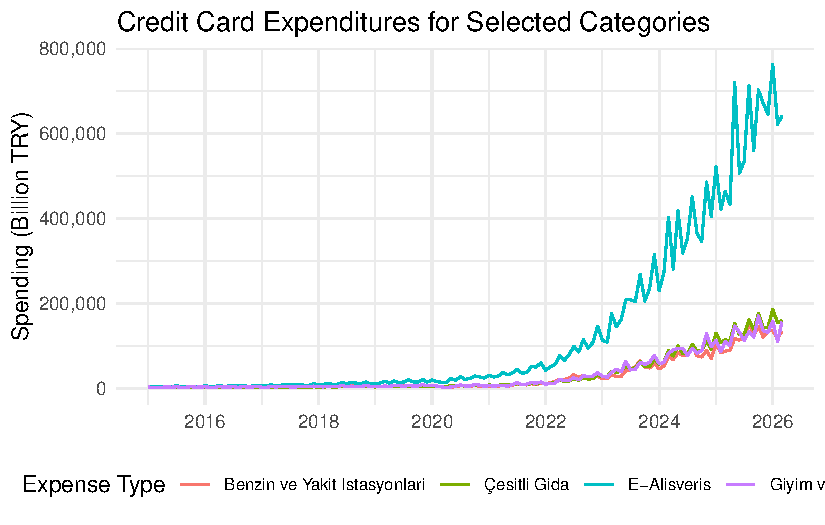
\includegraphics[keepaspectratio]{project_files/figure-pdf/unnamed-chunk-3-1.pdf}}
\end{itemize}

\subsubsection{Credit Card Expenditure
Table}\label{credit-card-expenditure-table}

\begin{itemize}
\item
  \textbf{Description}:
\item
  This table contains Year, Month, Expense Type, and Quantity.\\
\item
  Expense Type identifies the spending category, and Quantity gives the
  corresponding spending amount for that month.
\item
  This table contains sectoral spending amounts derived from credit card
  transactions.
\item
  The values in this table are expected to differ substantially across
  categories. Some categories such as retail, food, fuel, and e-commerce
  are likely to have much larger values than others.

\begin{Shaded}
\begin{Highlighting}[]
\FunctionTok{library}\NormalTok{(dplyr)}
\FunctionTok{library}\NormalTok{(ggplot2)}
\FunctionTok{library}\NormalTok{(scales)}
\NormalTok{expense\_quantity }\OtherTok{\textless{}{-}}\NormalTok{ Expense\_Quantity }\SpecialCharTok{\%\textgreater{}\%}
  \FunctionTok{filter}\NormalTok{(Year }\SpecialCharTok{\textless{}} \DecValTok{2026}\NormalTok{) }\SpecialCharTok{\%\textgreater{}\%}
  \FunctionTok{mutate}\NormalTok{(}\AttributeTok{Date =} \FunctionTok{as.Date}\NormalTok{(}\FunctionTok{sprintf}\NormalTok{(}\StringTok{"\%d{-}\%02d{-}01"}\NormalTok{, Year, Month)))}

\FunctionTok{ggplot}\NormalTok{(}
\NormalTok{  expense\_quantity }\SpecialCharTok{\%\textgreater{}\%}
    \FunctionTok{filter}\NormalTok{(Expense\_Type }\SpecialCharTok{\%in\%} \FunctionTok{c}\NormalTok{(}\StringTok{"E{-}Alışveriş"}\NormalTok{, }\StringTok{"Çeşitli Gıda"}\NormalTok{, }\StringTok{"Giyim ve Aksesuar"}\NormalTok{, }\StringTok{"Benzin ve Yakıt İstasyonları"}\NormalTok{)),}
  \FunctionTok{aes}\NormalTok{(}\AttributeTok{x =}\NormalTok{ Date, }\AttributeTok{y =}\NormalTok{ Quantity }\SpecialCharTok{/} \FloatTok{1e3}\NormalTok{, }\AttributeTok{color =}\NormalTok{ Expense\_Type)}
\NormalTok{) }\SpecialCharTok{+}
  \FunctionTok{geom\_line}\NormalTok{() }\SpecialCharTok{+}
  \FunctionTok{scale\_x\_date}\NormalTok{(}\AttributeTok{date\_breaks =} \StringTok{"2 years"}\NormalTok{, }\AttributeTok{date\_labels =} \StringTok{"\%Y"}\NormalTok{) }\SpecialCharTok{+}
  \FunctionTok{scale\_y\_continuous}\NormalTok{(}\AttributeTok{labels =} \FunctionTok{label\_comma}\NormalTok{(}\AttributeTok{accuracy =} \DecValTok{1}\NormalTok{)) }\SpecialCharTok{+}
  \FunctionTok{labs}\NormalTok{(}
    \AttributeTok{title =} \StringTok{"Credit Card Expenditures for Selected Categories"}\NormalTok{,}
    \AttributeTok{x =} \ConstantTok{NULL}\NormalTok{,}
    \AttributeTok{y =} \StringTok{"Spending (Billion TRY)"}\NormalTok{,}
    \AttributeTok{color =} \StringTok{"Expense Type"}
\NormalTok{  ) }\SpecialCharTok{+}
  \FunctionTok{theme\_minimal}\NormalTok{() }\SpecialCharTok{+}
  \FunctionTok{theme}\NormalTok{(}\AttributeTok{legend.position =} \StringTok{"bottom"}\NormalTok{,}
        \AttributeTok{legend.text =} \FunctionTok{element\_text}\NormalTok{(}\AttributeTok{size =} \DecValTok{8}\NormalTok{))}
\end{Highlighting}
\end{Shaded}

  \pandocbounded{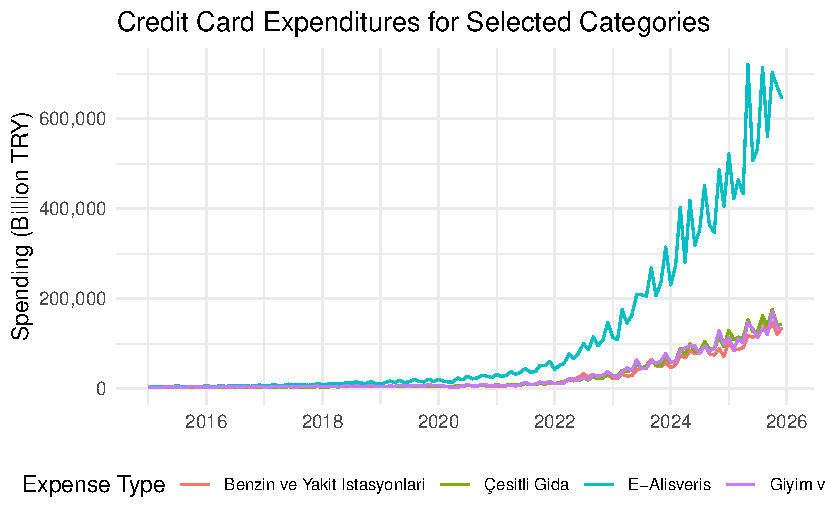
\includegraphics[keepaspectratio]{project_files/figure-pdf/unnamed-chunk-4-1.pdf}}
\end{itemize}

\subsubsection{Housing Panel Dataset}\label{housing-panel-dataset}

\begin{itemize}
\item
  \textbf{Description}:\\
  This is the main table for the project and contains Year, Month,
  Region, House Price Index, and Total Sales.

  Region represents the housing price index regions as in NUTS2 level,
  House Price Index shows the monthly house price index for that region,
  and Total Sales gives the aggregated monthly house sales value for the
  same region.

\begin{Shaded}
\begin{Highlighting}[]
\FunctionTok{library}\NormalTok{(dplyr)}
\FunctionTok{library}\NormalTok{(ggplot2)}
\FunctionTok{library}\NormalTok{(scales)}

\NormalTok{konut\_index\_sales }\OtherTok{\textless{}{-}}\NormalTok{ Konut\_Index\_Sales }\SpecialCharTok{\%\textgreater{}\%}
  \FunctionTok{filter}\NormalTok{(Year }\SpecialCharTok{\textless{}} \DecValTok{2026}\NormalTok{) }\SpecialCharTok{\%\textgreater{}\%}
  \FunctionTok{mutate}\NormalTok{(}\AttributeTok{Date =} \FunctionTok{as.Date}\NormalTok{(}\FunctionTok{sprintf}\NormalTok{(}\StringTok{"\%d{-}\%02d{-}01"}\NormalTok{, Year, Month)))}

\FunctionTok{ggplot}\NormalTok{(}
\NormalTok{  konut\_index\_sales }\SpecialCharTok{\%\textgreater{}\%} \FunctionTok{filter}\NormalTok{(Region }\SpecialCharTok{==} \StringTok{"Türkiye"}\NormalTok{),}
  \FunctionTok{aes}\NormalTok{(}\AttributeTok{x =}\NormalTok{ Date, }\AttributeTok{y =}\NormalTok{ Konut\_Endeksi)}
\NormalTok{) }\SpecialCharTok{+}
  \FunctionTok{geom\_line}\NormalTok{() }\SpecialCharTok{+}
  \FunctionTok{scale\_x\_date}\NormalTok{(}\AttributeTok{date\_breaks =} \StringTok{"2 years"}\NormalTok{, }\AttributeTok{date\_labels =} \StringTok{"\%Y"}\NormalTok{) }\SpecialCharTok{+}
  \FunctionTok{scale\_y\_continuous}\NormalTok{(}\AttributeTok{labels =} \FunctionTok{label\_comma}\NormalTok{(}\AttributeTok{accuracy =} \DecValTok{1}\NormalTok{)) }\SpecialCharTok{+}
  \FunctionTok{labs}\NormalTok{(}
    \AttributeTok{title =} \StringTok{"House Price Index in Türkiye Over Time"}\NormalTok{,}
    \AttributeTok{x =} \ConstantTok{NULL}\NormalTok{,}
    \AttributeTok{y =} \StringTok{"House Price Index"}
\NormalTok{  ) }\SpecialCharTok{+}
  \FunctionTok{theme\_minimal}\NormalTok{()}
\end{Highlighting}
\end{Shaded}

  \pandocbounded{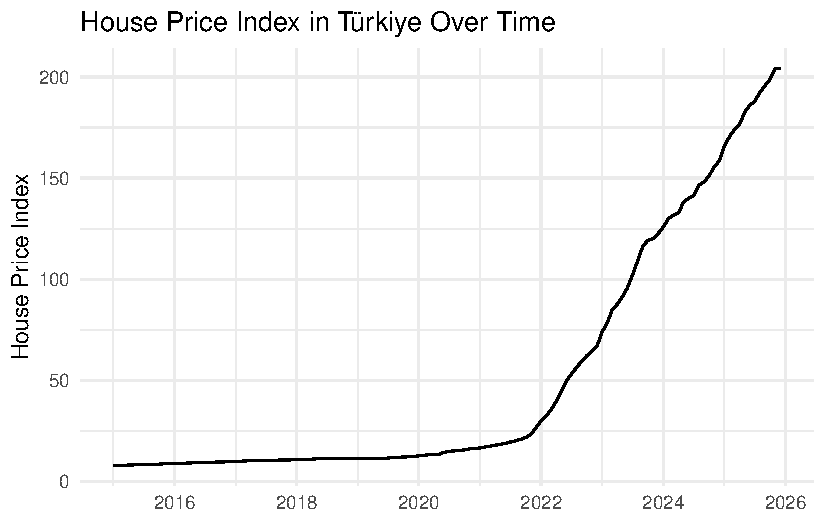
\includegraphics[keepaspectratio]{project_files/figure-pdf/unnamed-chunk-5-1.pdf}}
\end{itemize}

\begin{Shaded}
\begin{Highlighting}[]
\FunctionTok{library}\NormalTok{(dplyr)}
\FunctionTok{library}\NormalTok{(ggplot2)}
\FunctionTok{library}\NormalTok{(scales)}

\FunctionTok{ggplot}\NormalTok{(}
\NormalTok{  Konut\_Index\_Sales }\SpecialCharTok{\%\textgreater{}\%}
    \FunctionTok{filter}\NormalTok{(Year }\SpecialCharTok{\textless{}} \DecValTok{2026}\NormalTok{) }\SpecialCharTok{\%\textgreater{}\%}
    \FunctionTok{mutate}\NormalTok{(}\AttributeTok{Date =} \FunctionTok{as.Date}\NormalTok{(}\FunctionTok{sprintf}\NormalTok{(}\StringTok{"\%d{-}\%02d{-}01"}\NormalTok{, Year, Month))) }\SpecialCharTok{\%\textgreater{}\%}
    \FunctionTok{filter}\NormalTok{(Region }\SpecialCharTok{\%in\%} \FunctionTok{c}\NormalTok{(}\StringTok{"Türkiye"}\NormalTok{, }\StringTok{"İstanbul"}\NormalTok{, }\StringTok{"İzmir"}\NormalTok{, }\StringTok{"Ankara"}\NormalTok{, }\StringTok{"Adana, Mersin"}\NormalTok{)),}
  \FunctionTok{aes}\NormalTok{(}\AttributeTok{x =}\NormalTok{ Date, }\AttributeTok{y =}\NormalTok{ Total\_Sales, }\AttributeTok{color =}\NormalTok{ Region)}
\NormalTok{) }\SpecialCharTok{+}
  \FunctionTok{geom\_line}\NormalTok{() }\SpecialCharTok{+}
  \FunctionTok{scale\_x\_date}\NormalTok{(}\AttributeTok{date\_breaks =} \StringTok{"2 years"}\NormalTok{, }\AttributeTok{date\_labels =} \StringTok{"\%Y"}\NormalTok{) }\SpecialCharTok{+}
  \FunctionTok{scale\_y\_continuous}\NormalTok{(}\AttributeTok{labels =} \FunctionTok{label\_comma}\NormalTok{(}\AttributeTok{accuracy =} \DecValTok{1}\NormalTok{)) }\SpecialCharTok{+}
  \FunctionTok{labs}\NormalTok{(}
    \AttributeTok{title =} \StringTok{"Total House Sales for Selected Regions"}\NormalTok{,}
    \AttributeTok{x =} \ConstantTok{NULL}\NormalTok{,}
    \AttributeTok{y =} \StringTok{"Units Sold"}\NormalTok{,}
    \AttributeTok{color =} \StringTok{"Region"}
\NormalTok{  ) }\SpecialCharTok{+}
  \FunctionTok{theme\_minimal}\NormalTok{() }\SpecialCharTok{+}
  \FunctionTok{theme}\NormalTok{(}\AttributeTok{legend.position =} \StringTok{"bottom"}\NormalTok{)}
\end{Highlighting}
\end{Shaded}

\pandocbounded{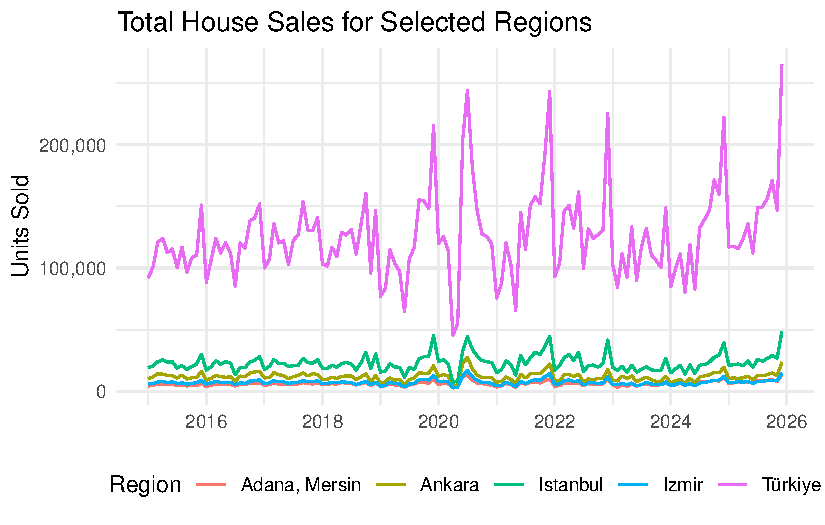
\includegraphics[keepaspectratio]{project_files/figure-pdf/unnamed-chunk-6-1.pdf}}

\subsection{Potential Analyses}\label{potential-analyses}

\begin{itemize}
\tightlist
\item
  time-series plots of house prices, exchange rates, and sales,
\item
  regional comparisons of house price growth,
\item
  correlations between exchange rates and the house price index,
\item
  relationships between sales volume and housing prices,
\item
  category-based spending trends over time,
\end{itemize}

\subsection{Reason of Choice}\label{reason-of-choice}

Housing prices are one of the most important economic and social issues
in Türkiye. The rapid increase in housing prices has significant
implications for affordability, investment decisions, and economic
stability.

All datasets are:

\begin{itemize}
\item
  Consistent in frequency (monthly)
\item
  Long enough for trend analysis
\item
  Rich enough for regional comparison

  This makes it easy for analyzing.
\end{itemize}

\subsection{Preprocessing}\label{preprocessing}

The raw EVDS datasets were provided in Excel format and contained
different structures (wide vs.~long) and aggregation levels (province
vs.~region). We performed preprocessing in Python using pandas to
standardize date formats, reshape wide datasets into long format, map
categorical codes to meaningful labels, and align all datasets at a
consistent monthly and regional level. In particular, house sales data
were converted from province-level columns to regional aggregates
compatible with the House Price Index. The final result consists of
three clean analytical tables ready for further analysis.

Another key issue was that EVDS datasets use \textbf{coded column names}
(e.g., \texttt{KT2}, \texttt{T58}, \texttt{TR62}) instead of descriptive
labels. To make the data interpretable and consistent across sources, we
created mapping dictionaries in Python to translate these codes into
meaningful categories, provinces, and regions.

Here you can find our python code.\\
\strut \\

\begin{Shaded}
\begin{Highlighting}[]
\CommentTok{\# We explained the data and the output tables to AI. It gave us this code\textquotesingle{}s first version. Then we fixed it according to our needs}
\ImportTok{import}\NormalTok{ pandas }\ImportTok{as}\NormalTok{ pd}
\ImportTok{from}\NormalTok{ pathlib }\ImportTok{import}\NormalTok{ Path}

\NormalTok{downloads }\OperatorTok{=}\NormalTok{ Path.home() }\OperatorTok{/} \StringTok{"Downloads"}

\CommentTok{\# Files}
\NormalTok{kurlar\_file }\OperatorTok{=}\NormalTok{ downloads }\OperatorTok{/} \StringTok{"Kurlar.xlsx"}
\NormalTok{kredi\_file }\OperatorTok{=}\NormalTok{ downloads }\OperatorTok{/} \StringTok{"Kredi Harcama.xlsx"}
\NormalTok{konut\_satis\_file }\OperatorTok{=}\NormalTok{ downloads }\OperatorTok{/} \StringTok{"Konut Satış.xlsx"}
\NormalTok{konut\_fiyat\_file }\OperatorTok{=}\NormalTok{ downloads }\OperatorTok{/} \StringTok{"Konut Fiyat Endexi.xlsx"}

\NormalTok{output\_file }\OperatorTok{=}\NormalTok{ downloads }\OperatorTok{/} \StringTok{"evds\_preprocessed\_tables\_fixed.xlsx"}

\CommentTok{\# {-}{-}{-}{-}{-}{-}{-}{-}{-}{-}{-}{-}{-}{-}{-}{-}{-}{-}{-}{-}{-}{-}{-}{-}{-}{-}{-}{-}{-}}
\CommentTok{\# Helper}
\CommentTok{\# {-}{-}{-}{-}{-}{-}{-}{-}{-}{-}{-}{-}{-}{-}{-}{-}{-}{-}{-}{-}{-}{-}{-}{-}{-}{-}{-}{-}{-}}
\KeywordTok{def}\NormalTok{ split\_year\_month(df):}
\NormalTok{    df[}\StringTok{"Tarih"}\NormalTok{] }\OperatorTok{=}\NormalTok{ pd.to\_datetime(df[}\StringTok{"Tarih"}\NormalTok{], }\BuiltInTok{format}\OperatorTok{=}\StringTok{"\%Y{-}\%m"}\NormalTok{)}
\NormalTok{    df[}\StringTok{"Year"}\NormalTok{] }\OperatorTok{=}\NormalTok{ df[}\StringTok{"Tarih"}\NormalTok{].dt.year}
\NormalTok{    df[}\StringTok{"Month"}\NormalTok{] }\OperatorTok{=}\NormalTok{ df[}\StringTok{"Tarih"}\NormalTok{].dt.month}
    \ControlFlowTok{return}\NormalTok{ df}

\CommentTok{\# {-}{-}{-}{-}{-}{-}{-}{-}{-}{-}{-}{-}{-}{-}{-}{-}{-}{-}{-}{-}{-}{-}{-}{-}{-}{-}{-}{-}{-}}
\CommentTok{\# Read}
\CommentTok{\# {-}{-}{-}{-}{-}{-}{-}{-}{-}{-}{-}{-}{-}{-}{-}{-}{-}{-}{-}{-}{-}{-}{-}{-}{-}{-}{-}{-}{-}}
\NormalTok{kurlar }\OperatorTok{=}\NormalTok{ split\_year\_month(pd.read\_excel(kurlar\_file))}
\NormalTok{kredi }\OperatorTok{=}\NormalTok{ split\_year\_month(pd.read\_excel(kredi\_file))}
\NormalTok{satis }\OperatorTok{=}\NormalTok{ split\_year\_month(pd.read\_excel(konut\_satis\_file))}
\NormalTok{kfe }\OperatorTok{=}\NormalTok{ split\_year\_month(pd.read\_excel(konut\_fiyat\_file))}

\CommentTok{\# {-}{-}{-}{-}{-}{-}{-}{-}{-}{-}{-}{-}{-}{-}{-}{-}{-}{-}{-}{-}{-}{-}{-}{-}{-}{-}{-}{-}{-}}
\CommentTok{\# TABLE 1: Exchange Rates}
\CommentTok{\# {-}{-}{-}{-}{-}{-}{-}{-}{-}{-}{-}{-}{-}{-}{-}{-}{-}{-}{-}{-}{-}{-}{-}{-}{-}{-}{-}{-}{-}}
\NormalTok{table\_kurlar }\OperatorTok{=}\NormalTok{ (}
\NormalTok{    kurlar[[}\StringTok{"Year"}\NormalTok{, }\StringTok{"Month"}\NormalTok{, }\StringTok{"TP\_DK\_USD\_S\_YTL"}\NormalTok{, }\StringTok{"TP\_DK\_EUR\_S\_YTL"}\NormalTok{]]}
\NormalTok{    .rename(columns}\OperatorTok{=}\NormalTok{\{}
        \StringTok{"TP\_DK\_USD\_S\_YTL"}\NormalTok{: }\StringTok{"USD"}\NormalTok{,}
        \StringTok{"TP\_DK\_EUR\_S\_YTL"}\NormalTok{: }\StringTok{"EUR"}
\NormalTok{    \})}
\NormalTok{)}

\CommentTok{\# {-}{-}{-}{-}{-}{-}{-}{-}{-}{-}{-}{-}{-}{-}{-}{-}{-}{-}{-}{-}{-}{-}{-}{-}{-}{-}{-}{-}{-}}
\CommentTok{\# TABLE 2: Credit Expenditures}
\CommentTok{\# {-}{-}{-}{-}{-}{-}{-}{-}{-}{-}{-}{-}{-}{-}{-}{-}{-}{-}{-}{-}{-}{-}{-}{-}{-}{-}{-}{-}{-}}
\NormalTok{expense\_type\_map }\OperatorTok{=}\NormalTok{ \{}
    \StringTok{"TP\_KKHARTUT\_KT2"}\NormalTok{: }\StringTok{"Car Rental"}\NormalTok{,}
    \StringTok{"TP\_KKHARTUT\_KT3"}\NormalTok{: }\StringTok{"Car Sales/Service"}\NormalTok{,}
    \StringTok{"TP\_KKHARTUT\_KT4"}\NormalTok{: }\StringTok{"Fuel"}\NormalTok{,}
    \StringTok{"TP\_KKHARTUT\_KT5"}\NormalTok{: }\StringTok{"Food"}\NormalTok{,}
    \StringTok{"TP\_KKHARTUT\_KT6"}\NormalTok{: }\StringTok{"Direct Marketing"}\NormalTok{,}
    \StringTok{"TP\_KKHARTUT\_KT7"}\NormalTok{: }\StringTok{"Education"}\NormalTok{,}
    \StringTok{"TP\_KKHARTUT\_KT8"}\NormalTok{: }\StringTok{"Electronics"}\NormalTok{,}
    \StringTok{"TP\_KKHARTUT\_KT9"}\NormalTok{: }\StringTok{"Clothing"}\NormalTok{,}
    \StringTok{"TP\_KKHARTUT\_KT10"}\NormalTok{: }\StringTok{"Airlines"}\NormalTok{,}
    \StringTok{"TP\_KKHARTUT\_KT11"}\NormalTok{: }\StringTok{"Services"}\NormalTok{,}
    \StringTok{"TP\_KKHARTUT\_KT12"}\NormalTok{: }\StringTok{"Accommodation"}\NormalTok{,}
    \StringTok{"TP\_KKHARTUT\_KT13"}\NormalTok{: }\StringTok{"Social"}\NormalTok{,}
    \StringTok{"TP\_KKHARTUT\_KT14"}\NormalTok{: }\StringTok{"Entertainment"}\NormalTok{,}
    \StringTok{"TP\_KKHARTUT\_KT15"}\NormalTok{: }\StringTok{"Jewelry"}\NormalTok{,}
    \StringTok{"TP\_KKHARTUT\_KT16"}\NormalTok{: }\StringTok{"Retail"}\NormalTok{,}
    \StringTok{"TP\_KKHARTUT\_KT17"}\NormalTok{: }\StringTok{"Furniture"}\NormalTok{,}
    \StringTok{"TP\_KKHARTUT\_KT18"}\NormalTok{: }\StringTok{"Construction"}\NormalTok{,}
    \StringTok{"TP\_KKHARTUT\_KT19"}\NormalTok{: }\StringTok{"Health"}\NormalTok{,}
    \StringTok{"TP\_KKHARTUT\_KT20"}\NormalTok{: }\StringTok{"Travel"}\NormalTok{,}
    \StringTok{"TP\_KKHARTUT\_KT21"}\NormalTok{: }\StringTok{"Insurance"}\NormalTok{,}
    \StringTok{"TP\_KKHARTUT\_KT22"}\NormalTok{: }\StringTok{"Telecom"}\NormalTok{,}
    \StringTok{"TP\_KKHARTUT\_KT23"}\NormalTok{: }\StringTok{"Hardware"}\NormalTok{,}
    \StringTok{"TP\_KKHARTUT\_KT24"}\NormalTok{: }\StringTok{"Food Service"}\NormalTok{,}
    \StringTok{"TP\_KKHARTUT\_KT25"}\NormalTok{: }\StringTok{"Misc"}\NormalTok{,}
    \StringTok{"TP\_KKHARTUT\_KT26"}\NormalTok{: }\StringTok{"Other"}\NormalTok{,}
    \StringTok{"TP\_KKHARTUT\_KT50"}\NormalTok{: }\StringTok{"E{-}Commerce"}
\NormalTok{\}}

\NormalTok{kredi\_cols }\OperatorTok{=}\NormalTok{ [c }\ControlFlowTok{for}\NormalTok{ c }\KeywordTok{in}\NormalTok{ expense\_type\_map }\ControlFlowTok{if}\NormalTok{ c }\KeywordTok{in}\NormalTok{ kredi.columns]}

\NormalTok{table\_kredi }\OperatorTok{=}\NormalTok{ (}
\NormalTok{    kredi.melt(}
\NormalTok{        id\_vars}\OperatorTok{=}\NormalTok{[}\StringTok{"Year"}\NormalTok{, }\StringTok{"Month"}\NormalTok{],}
\NormalTok{        value\_vars}\OperatorTok{=}\NormalTok{kredi\_cols,}
\NormalTok{        var\_name}\OperatorTok{=}\StringTok{"Code"}\NormalTok{,}
\NormalTok{        value\_name}\OperatorTok{=}\StringTok{"Quantity"}
\NormalTok{    )}
\NormalTok{    .assign(Expense\_Type}\OperatorTok{=}\KeywordTok{lambda}\NormalTok{ x: x[}\StringTok{"Code"}\NormalTok{].}\BuiltInTok{map}\NormalTok{(expense\_type\_map))}
\NormalTok{    [[}\StringTok{"Year"}\NormalTok{, }\StringTok{"Month"}\NormalTok{, }\StringTok{"Expense\_Type"}\NormalTok{, }\StringTok{"Quantity"}\NormalTok{]]}
\NormalTok{)}

\CommentTok{\# {-}{-}{-}{-}{-}{-}{-}{-}{-}{-}{-}{-}{-}{-}{-}{-}{-}{-}{-}{-}{-}{-}{-}{-}{-}{-}{-}{-}{-}}
\CommentTok{\# TABLE 3: Housing Panel}
\CommentTok{\# {-}{-}{-}{-}{-}{-}{-}{-}{-}{-}{-}{-}{-}{-}{-}{-}{-}{-}{-}{-}{-}{-}{-}{-}{-}{-}{-}{-}{-}}
\NormalTok{provinces }\OperatorTok{=}\NormalTok{ [}
    \StringTok{"Adana"}\NormalTok{,}\StringTok{"Adıyaman"}\NormalTok{,}\StringTok{"Afyonkarahisar"}\NormalTok{,}\StringTok{"Ağrı"}\NormalTok{,}\StringTok{"Aksaray"}\NormalTok{,}\StringTok{"Amasya"}\NormalTok{,}\StringTok{"Ankara"}\NormalTok{,}
    \StringTok{"Antalya"}\NormalTok{,}\StringTok{"Ardahan"}\NormalTok{,}\StringTok{"Artvin"}\NormalTok{,}\StringTok{"Aydın"}\NormalTok{,}\StringTok{"Balıkesir"}\NormalTok{,}\StringTok{"Bartın"}\NormalTok{,}\StringTok{"Batman"}\NormalTok{,}
    \StringTok{"Bayburt"}\NormalTok{,}\StringTok{"Bilecik"}\NormalTok{,}\StringTok{"Bingöl"}\NormalTok{,}\StringTok{"Bitlis"}\NormalTok{,}\StringTok{"Bolu"}\NormalTok{,}\StringTok{"Burdur"}\NormalTok{,}\StringTok{"Bursa"}\NormalTok{,}\StringTok{"Çanakkale"}\NormalTok{,}
    \StringTok{"Çankırı"}\NormalTok{,}\StringTok{"Çorum"}\NormalTok{,}\StringTok{"Denizli"}\NormalTok{,}\StringTok{"Diyarbakır"}\NormalTok{,}\StringTok{"Düzce"}\NormalTok{,}\StringTok{"Edirne"}\NormalTok{,}\StringTok{"Elazığ"}\NormalTok{,}
    \StringTok{"Erzincan"}\NormalTok{,}\StringTok{"Erzurum"}\NormalTok{,}\StringTok{"Eskişehir"}\NormalTok{,}\StringTok{"Gaziantep"}\NormalTok{,}\StringTok{"Giresun"}\NormalTok{,}\StringTok{"Gümüşhane"}\NormalTok{,}
    \StringTok{"Hakkâri"}\NormalTok{,}\StringTok{"Hatay"}\NormalTok{,}\StringTok{"Iğdır"}\NormalTok{,}\StringTok{"Isparta"}\NormalTok{,}\StringTok{"İstanbul"}\NormalTok{,}\StringTok{"İzmir"}\NormalTok{,}\StringTok{"Kahramanmaraş"}\NormalTok{,}
    \StringTok{"Karabük"}\NormalTok{,}\StringTok{"Karaman"}\NormalTok{,}\StringTok{"Kars"}\NormalTok{,}\StringTok{"Kastamonu"}\NormalTok{,}\StringTok{"Kayseri"}\NormalTok{,}\StringTok{"Kırıkkale"}\NormalTok{,}\StringTok{"Kırklareli"}\NormalTok{,}
    \StringTok{"Kırşehir"}\NormalTok{,}\StringTok{"Kilis"}\NormalTok{,}\StringTok{"Kocaeli"}\NormalTok{,}\StringTok{"Konya"}\NormalTok{,}\StringTok{"Kütahya"}\NormalTok{,}\StringTok{"Malatya"}\NormalTok{,}\StringTok{"Manisa"}\NormalTok{,}
    \StringTok{"Mardin"}\NormalTok{,}\StringTok{"Mersin"}\NormalTok{,}\StringTok{"Muğla"}\NormalTok{,}\StringTok{"Muş"}\NormalTok{,}\StringTok{"Nevşehir"}\NormalTok{,}\StringTok{"Niğde"}\NormalTok{,}\StringTok{"Ordu"}\NormalTok{,}\StringTok{"Osmaniye"}\NormalTok{,}
    \StringTok{"Rize"}\NormalTok{,}\StringTok{"Sakarya"}\NormalTok{,}\StringTok{"Samsun"}\NormalTok{,}\StringTok{"Siirt"}\NormalTok{,}\StringTok{"Sinop"}\NormalTok{,}\StringTok{"Sivas"}\NormalTok{,}\StringTok{"Şanlıurfa"}\NormalTok{,}\StringTok{"Şırnak"}\NormalTok{,}
    \StringTok{"Tekirdağ"}\NormalTok{,}\StringTok{"Tokat"}\NormalTok{,}\StringTok{"Trabzon"}\NormalTok{,}\StringTok{"Tunceli"}\NormalTok{,}\StringTok{"Uşak"}\NormalTok{,}\StringTok{"Van"}\NormalTok{,}\StringTok{"Yalova"}\NormalTok{,}\StringTok{"Yozgat"}\NormalTok{,}
    \StringTok{"Zonguldak"}
\NormalTok{]}

\NormalTok{code\_map }\OperatorTok{=}\NormalTok{ \{}\StringTok{"TP\_AKONUTSAT1\_K1"}\NormalTok{: provinces[}\DecValTok{0}\NormalTok{]\}}
\ControlFlowTok{for}\NormalTok{ i }\KeywordTok{in} \BuiltInTok{range}\NormalTok{(}\DecValTok{2}\NormalTok{, }\DecValTok{82}\NormalTok{):}
\NormalTok{    code\_map[}\SpecialStringTok{f"TP\_AKONUTSAT1\_T}\SpecialCharTok{\{}\NormalTok{i}\SpecialCharTok{\}}\SpecialStringTok{"}\NormalTok{] }\OperatorTok{=}\NormalTok{ provinces[i}\OperatorTok{{-}}\DecValTok{1}\NormalTok{]}

\NormalTok{sales\_cols }\OperatorTok{=}\NormalTok{ [c }\ControlFlowTok{for}\NormalTok{ c }\KeywordTok{in}\NormalTok{ satis.columns }\ControlFlowTok{if}\NormalTok{ c }\KeywordTok{in}\NormalTok{ code\_map]}

\NormalTok{sales\_long }\OperatorTok{=}\NormalTok{ (}
\NormalTok{    satis.melt(}
\NormalTok{        id\_vars}\OperatorTok{=}\NormalTok{[}\StringTok{"Year"}\NormalTok{, }\StringTok{"Month"}\NormalTok{],}
\NormalTok{        value\_vars}\OperatorTok{=}\NormalTok{sales\_cols,}
\NormalTok{        var\_name}\OperatorTok{=}\StringTok{"Code"}\NormalTok{,}
\NormalTok{        value\_name}\OperatorTok{=}\StringTok{"Sales"}
\NormalTok{    )}
\NormalTok{    .assign(Province}\OperatorTok{=}\KeywordTok{lambda}\NormalTok{ x: x[}\StringTok{"Code"}\NormalTok{].}\BuiltInTok{map}\NormalTok{(code\_map))}
\NormalTok{)}

\CommentTok{\# Region mapping (example simplified)}
\NormalTok{region\_map }\OperatorTok{=}\NormalTok{ \{}
    \StringTok{"Adana"}\NormalTok{:}\StringTok{"TR62"}\NormalTok{,}\StringTok{"Mersin"}\NormalTok{:}\StringTok{"TR62"}\NormalTok{,}\StringTok{"Ankara"}\NormalTok{:}\StringTok{"TR51"}\NormalTok{,}\StringTok{"İstanbul"}\NormalTok{:}\StringTok{"TR10"}
\NormalTok{\}}

\NormalTok{sales\_long[}\StringTok{"Region\_Code"}\NormalTok{] }\OperatorTok{=}\NormalTok{ sales\_long[}\StringTok{"Province"}\NormalTok{].}\BuiltInTok{map}\NormalTok{(region\_map)}

\NormalTok{sales\_region }\OperatorTok{=}\NormalTok{ (}
\NormalTok{    sales\_long.groupby([}\StringTok{"Year"}\NormalTok{,}\StringTok{"Month"}\NormalTok{,}\StringTok{"Region\_Code"}\NormalTok{])[}\StringTok{"Sales"}\NormalTok{].}\BuiltInTok{sum}\NormalTok{().reset\_index()}
\NormalTok{)}

\NormalTok{kfe\_map }\OperatorTok{=}\NormalTok{ \{}
    \StringTok{"TP\_KFE\_TR62"}\NormalTok{:}\StringTok{"TR62"}\NormalTok{,}
    \StringTok{"TP\_KFE\_TR51"}\NormalTok{:}\StringTok{"TR51"}\NormalTok{,}
    \StringTok{"TP\_KFE\_TR10"}\NormalTok{:}\StringTok{"TR10"}
\NormalTok{\}}

\NormalTok{kfe\_cols }\OperatorTok{=}\NormalTok{ [c }\ControlFlowTok{for}\NormalTok{ c }\KeywordTok{in}\NormalTok{ kfe\_map }\ControlFlowTok{if}\NormalTok{ c }\KeywordTok{in}\NormalTok{ kfe.columns]}

\NormalTok{kfe\_long }\OperatorTok{=}\NormalTok{ (}
\NormalTok{    kfe.melt(}
\NormalTok{        id\_vars}\OperatorTok{=}\NormalTok{[}\StringTok{"Year"}\NormalTok{,}\StringTok{"Month"}\NormalTok{],}
\NormalTok{        value\_vars}\OperatorTok{=}\NormalTok{kfe\_cols,}
\NormalTok{        var\_name}\OperatorTok{=}\StringTok{"Code"}\NormalTok{,}
\NormalTok{        value\_name}\OperatorTok{=}\StringTok{"House\_Price\_Index"}
\NormalTok{    )}
\NormalTok{    .assign(Region\_Code}\OperatorTok{=}\KeywordTok{lambda}\NormalTok{ x: x[}\StringTok{"Code"}\NormalTok{].}\BuiltInTok{map}\NormalTok{(kfe\_map))}
\NormalTok{)}

\NormalTok{table\_konut }\OperatorTok{=}\NormalTok{ kfe\_long.merge(}
\NormalTok{    sales\_region,}
\NormalTok{    on}\OperatorTok{=}\NormalTok{[}\StringTok{"Year"}\NormalTok{,}\StringTok{"Month"}\NormalTok{,}\StringTok{"Region\_Code"}\NormalTok{]}
\NormalTok{)}

\CommentTok{\# {-}{-}{-}{-}{-}{-}{-}{-}{-}{-}{-}{-}{-}{-}{-}{-}{-}{-}{-}{-}{-}{-}{-}{-}{-}{-}{-}{-}{-}}
\CommentTok{\# SAVE}
\CommentTok{\# {-}{-}{-}{-}{-}{-}{-}{-}{-}{-}{-}{-}{-}{-}{-}{-}{-}{-}{-}{-}{-}{-}{-}{-}{-}{-}{-}{-}{-}}
\ControlFlowTok{with}\NormalTok{ pd.ExcelWriter(output\_file) }\ImportTok{as}\NormalTok{ writer:}
\NormalTok{    table\_kurlar.to\_excel(writer, sheet\_name}\OperatorTok{=}\StringTok{"USD\_EUR"}\NormalTok{, index}\OperatorTok{=}\VariableTok{False}\NormalTok{)}
\NormalTok{    table\_kredi.to\_excel(writer, sheet\_name}\OperatorTok{=}\StringTok{"Expense"}\NormalTok{, index}\OperatorTok{=}\VariableTok{False}\NormalTok{)}
\NormalTok{    table\_konut.to\_excel(writer, sheet\_name}\OperatorTok{=}\StringTok{"Housing"}\NormalTok{, index}\OperatorTok{=}\VariableTok{False}\NormalTok{)}
\end{Highlighting}
\end{Shaded}

\section{Analysis}\label{analysis}

\begin{Shaded}
\begin{Highlighting}[]
\FunctionTok{library}\NormalTok{(dplyr)}
\FunctionTok{library}\NormalTok{(ggplot2)}
\FunctionTok{library}\NormalTok{(tidyr)}
\FunctionTok{library}\NormalTok{(scales)}
\FunctionTok{library}\NormalTok{(knitr)}
\FunctionTok{library}\NormalTok{(kableExtra)}

\FunctionTok{load}\NormalTok{(}\StringTok{"Project\_Data.RData"}\NormalTok{)}

\NormalTok{cr }\OtherTok{\textless{}{-}}\NormalTok{ Conversion\_Rates }\SpecialCharTok{\%\textgreater{}\%}
  \FunctionTok{filter}\NormalTok{(Year }\SpecialCharTok{\textless{}} \DecValTok{2026}\NormalTok{) }\SpecialCharTok{\%\textgreater{}\%}
  \FunctionTok{mutate}\NormalTok{(}\AttributeTok{Date =} \FunctionTok{as.Date}\NormalTok{(}\FunctionTok{sprintf}\NormalTok{(}\StringTok{"\%d{-}\%02d{-}01"}\NormalTok{, Year, Month)))}

\NormalTok{eq }\OtherTok{\textless{}{-}}\NormalTok{ Expense\_Quantity }\SpecialCharTok{\%\textgreater{}\%}
  \FunctionTok{filter}\NormalTok{(Year }\SpecialCharTok{\textless{}} \DecValTok{2026}\NormalTok{) }\SpecialCharTok{\%\textgreater{}\%}
  \FunctionTok{mutate}\NormalTok{(}\AttributeTok{Date =} \FunctionTok{as.Date}\NormalTok{(}\FunctionTok{sprintf}\NormalTok{(}\StringTok{"\%d{-}\%02d{-}01"}\NormalTok{, Year, Month)))}

\NormalTok{ks }\OtherTok{\textless{}{-}}\NormalTok{ Konut\_Index\_Sales }\SpecialCharTok{\%\textgreater{}\%}
  \FunctionTok{filter}\NormalTok{(Year }\SpecialCharTok{\textless{}} \DecValTok{2026}\NormalTok{) }\SpecialCharTok{\%\textgreater{}\%}
  \FunctionTok{mutate}\NormalTok{(}\AttributeTok{Date =} \FunctionTok{as.Date}\NormalTok{(}\FunctionTok{sprintf}\NormalTok{(}\StringTok{"\%d{-}\%02d{-}01"}\NormalTok{, Year, Month)))}

\NormalTok{ks\_turkey }\OtherTok{\textless{}{-}}\NormalTok{ ks }\SpecialCharTok{\%\textgreater{}\%} \FunctionTok{filter}\NormalTok{(Region }\SpecialCharTok{==} \StringTok{"Türkiye"}\NormalTok{)}

\CommentTok{\# Build the shared joined dataset used throughout Analysis}
\NormalTok{total\_cc }\OtherTok{\textless{}{-}}\NormalTok{ eq }\SpecialCharTok{\%\textgreater{}\%}
  \FunctionTok{group\_by}\NormalTok{(Year, Month) }\SpecialCharTok{\%\textgreater{}\%}
  \FunctionTok{summarise}\NormalTok{(}\AttributeTok{Total\_CC =} \FunctionTok{sum}\NormalTok{(Quantity, }\AttributeTok{na.rm =} \ConstantTok{TRUE}\NormalTok{), }\AttributeTok{.groups =} \StringTok{"drop"}\NormalTok{)}

\NormalTok{combined }\OtherTok{\textless{}{-}}\NormalTok{ ks\_turkey }\SpecialCharTok{\%\textgreater{}\%}
  \FunctionTok{inner\_join}\NormalTok{(cr }\SpecialCharTok{\%\textgreater{}\%} \FunctionTok{select}\NormalTok{(Year, Month, USD, EUR), }\AttributeTok{by =} \FunctionTok{c}\NormalTok{(}\StringTok{"Year"}\NormalTok{, }\StringTok{"Month"}\NormalTok{)) }\SpecialCharTok{\%\textgreater{}\%}
  \FunctionTok{inner\_join}\NormalTok{(total\_cc, }\AttributeTok{by =} \FunctionTok{c}\NormalTok{(}\StringTok{"Year"}\NormalTok{, }\StringTok{"Month"}\NormalTok{))}
\end{Highlighting}
\end{Shaded}

\subsection{Exploratory Data Analysis}\label{exploratory-data-analysis}

We begin by examining the basic descriptive statistics of each key
variable to understand their range and scale before looking at
relationships.

\begin{Shaded}
\begin{Highlighting}[]
\FunctionTok{bind\_rows}\NormalTok{(}
\NormalTok{  ks\_turkey }\SpecialCharTok{\%\textgreater{}\%} \FunctionTok{summarise}\NormalTok{(}
    \AttributeTok{Variable =} \StringTok{"House Price Index"}\NormalTok{,}
    \AttributeTok{Min      =} \FunctionTok{min}\NormalTok{(Konut\_Endeksi, }\AttributeTok{na.rm =} \ConstantTok{TRUE}\NormalTok{),}
    \AttributeTok{Mean     =} \FunctionTok{mean}\NormalTok{(Konut\_Endeksi, }\AttributeTok{na.rm =} \ConstantTok{TRUE}\NormalTok{),}
    \AttributeTok{Median   =} \FunctionTok{median}\NormalTok{(Konut\_Endeksi, }\AttributeTok{na.rm =} \ConstantTok{TRUE}\NormalTok{),}
    \AttributeTok{Max      =} \FunctionTok{max}\NormalTok{(Konut\_Endeksi, }\AttributeTok{na.rm =} \ConstantTok{TRUE}\NormalTok{),}
    \AttributeTok{SD       =} \FunctionTok{sd}\NormalTok{(Konut\_Endeksi, }\AttributeTok{na.rm =} \ConstantTok{TRUE}\NormalTok{)}
\NormalTok{  ),}
\NormalTok{  ks\_turkey }\SpecialCharTok{\%\textgreater{}\%} \FunctionTok{summarise}\NormalTok{(}
    \AttributeTok{Variable =} \StringTok{"Monthly Sales (units)"}\NormalTok{,}
    \AttributeTok{Min      =} \FunctionTok{min}\NormalTok{(Total\_Sales, }\AttributeTok{na.rm =} \ConstantTok{TRUE}\NormalTok{),}
    \AttributeTok{Mean     =} \FunctionTok{mean}\NormalTok{(Total\_Sales, }\AttributeTok{na.rm =} \ConstantTok{TRUE}\NormalTok{),}
    \AttributeTok{Median   =} \FunctionTok{median}\NormalTok{(Total\_Sales, }\AttributeTok{na.rm =} \ConstantTok{TRUE}\NormalTok{),}
    \AttributeTok{Max      =} \FunctionTok{max}\NormalTok{(Total\_Sales, }\AttributeTok{na.rm =} \ConstantTok{TRUE}\NormalTok{),}
    \AttributeTok{SD       =} \FunctionTok{sd}\NormalTok{(Total\_Sales, }\AttributeTok{na.rm =} \ConstantTok{TRUE}\NormalTok{)}
\NormalTok{  ),}
\NormalTok{  cr }\SpecialCharTok{\%\textgreater{}\%} \FunctionTok{summarise}\NormalTok{(}
    \AttributeTok{Variable =} \StringTok{"USD/TRY Rate"}\NormalTok{,}
    \AttributeTok{Min      =} \FunctionTok{min}\NormalTok{(USD, }\AttributeTok{na.rm =} \ConstantTok{TRUE}\NormalTok{),}
    \AttributeTok{Mean     =} \FunctionTok{mean}\NormalTok{(USD, }\AttributeTok{na.rm =} \ConstantTok{TRUE}\NormalTok{),}
    \AttributeTok{Median   =} \FunctionTok{median}\NormalTok{(USD, }\AttributeTok{na.rm =} \ConstantTok{TRUE}\NormalTok{),}
    \AttributeTok{Max      =} \FunctionTok{max}\NormalTok{(USD, }\AttributeTok{na.rm =} \ConstantTok{TRUE}\NormalTok{),}
    \AttributeTok{SD       =} \FunctionTok{sd}\NormalTok{(USD, }\AttributeTok{na.rm =} \ConstantTok{TRUE}\NormalTok{)}
\NormalTok{  ),}
\NormalTok{  cr }\SpecialCharTok{\%\textgreater{}\%} \FunctionTok{summarise}\NormalTok{(}
    \AttributeTok{Variable =} \StringTok{"EUR/TRY Rate"}\NormalTok{,}
    \AttributeTok{Min      =} \FunctionTok{min}\NormalTok{(EUR, }\AttributeTok{na.rm =} \ConstantTok{TRUE}\NormalTok{),}
    \AttributeTok{Mean     =} \FunctionTok{mean}\NormalTok{(EUR, }\AttributeTok{na.rm =} \ConstantTok{TRUE}\NormalTok{),}
    \AttributeTok{Median   =} \FunctionTok{median}\NormalTok{(EUR, }\AttributeTok{na.rm =} \ConstantTok{TRUE}\NormalTok{),}
    \AttributeTok{Max      =} \FunctionTok{max}\NormalTok{(EUR, }\AttributeTok{na.rm =} \ConstantTok{TRUE}\NormalTok{),}
    \AttributeTok{SD       =} \FunctionTok{sd}\NormalTok{(EUR, }\AttributeTok{na.rm =} \ConstantTok{TRUE}\NormalTok{)}
\NormalTok{  )}
\NormalTok{) }\SpecialCharTok{\%\textgreater{}\%}
  \FunctionTok{mutate}\NormalTok{(}\FunctionTok{across}\NormalTok{(}\FunctionTok{where}\NormalTok{(is.numeric), }\SpecialCharTok{\textasciitilde{}} \FunctionTok{format}\NormalTok{(}\FunctionTok{round}\NormalTok{(.x, }\DecValTok{1}\NormalTok{), }\AttributeTok{big.mark =} \StringTok{","}\NormalTok{))) }\SpecialCharTok{\%\textgreater{}\%}
  \FunctionTok{kable}\NormalTok{(}\AttributeTok{caption =} \StringTok{"Table 1. Summary Statistics of Key Variables"}\NormalTok{) }\SpecialCharTok{\%\textgreater{}\%}
  \FunctionTok{kable\_styling}\NormalTok{(}\AttributeTok{bootstrap\_options =} \FunctionTok{c}\NormalTok{(}\StringTok{"striped"}\NormalTok{, }\StringTok{"hover"}\NormalTok{), }\AttributeTok{full\_width =} \ConstantTok{FALSE}\NormalTok{)}
\end{Highlighting}
\end{Shaded}

\begin{longtable}[t]{llllll}
\caption{\label{tab:eda-summary}Table 1. Summary Statistics of Key Variables}\\
\toprule
Variable & Min & Mean & Median & Max & SD\\
\midrule
House Price Index & 7.7 & 51.1 & 14.6 & 204.4 & 60.8\\
Monthly Sales (units) & 45,218.0 & 126,140.7 & 120,437.5 & 265,223.0 & 35,718.6\\
USD/TRY Rate & 2.1 & 12.6 & 6.1 & 42.7 & 12.4\\
EUR/TRY Rate & 2.7 & 13.9 & 6.8 & 49.9 & 13.7\\
\bottomrule
\end{longtable}

The House Price Index increased from low initial values to several
thousand index points by the end of the sample period, showing the scale
of the housing price surge in Türkiye. The exchange rate variables also
rose sharply, while monthly sales remained volatile rather than
following the same continuous upward pattern. This first descriptive
comparison already suggests that price growth was more closely aligned
with macroeconomic nominal variables than with transaction volume.

\begin{Shaded}
\begin{Highlighting}[]
\NormalTok{eq }\SpecialCharTok{\%\textgreater{}\%}
  \FunctionTok{group\_by}\NormalTok{(Expense\_Type) }\SpecialCharTok{\%\textgreater{}\%}
  \FunctionTok{summarise}\NormalTok{(}\AttributeTok{Total\_Billion\_TRY =} \FunctionTok{sum}\NormalTok{(Quantity, }\AttributeTok{na.rm =} \ConstantTok{TRUE}\NormalTok{) }\SpecialCharTok{/} \FloatTok{1e3}\NormalTok{, }\AttributeTok{.groups =} \StringTok{"drop"}\NormalTok{) }\SpecialCharTok{\%\textgreater{}\%}
  \FunctionTok{arrange}\NormalTok{(}\FunctionTok{desc}\NormalTok{(Total\_Billion\_TRY)) }\SpecialCharTok{\%\textgreater{}\%}
  \FunctionTok{slice\_head}\NormalTok{(}\AttributeTok{n =} \DecValTok{8}\NormalTok{) }\SpecialCharTok{\%\textgreater{}\%}
  \FunctionTok{mutate}\NormalTok{(}\AttributeTok{Total\_Billion\_TRY =} \FunctionTok{format}\NormalTok{(}\FunctionTok{round}\NormalTok{(Total\_Billion\_TRY, }\DecValTok{0}\NormalTok{), }\AttributeTok{big.mark =} \StringTok{","}\NormalTok{)) }\SpecialCharTok{\%\textgreater{}\%}
  \FunctionTok{kable}\NormalTok{(}\AttributeTok{col.names =} \FunctionTok{c}\NormalTok{(}\StringTok{"Expense Category"}\NormalTok{, }\StringTok{"Total Spending (Billion TRY)"}\NormalTok{),}
        \AttributeTok{caption =} \StringTok{"Table 2. Top 8 Credit Card Expenditure Categories – Cumulative Total"}\NormalTok{) }\SpecialCharTok{\%\textgreater{}\%}
  \FunctionTok{kable\_styling}\NormalTok{(}\AttributeTok{bootstrap\_options =} \FunctionTok{c}\NormalTok{(}\StringTok{"striped"}\NormalTok{, }\StringTok{"hover"}\NormalTok{), }\AttributeTok{full\_width =} \ConstantTok{FALSE}\NormalTok{)}
\end{Highlighting}
\end{Shaded}

\begin{longtable}[t]{ll}
\caption{\label{tab:eda-credit-top}Table 2. Top 8 Credit Card Expenditure Categories – Cumulative Total}\\
\toprule
Expense Category & Total Spending (Billion TRY)\\
\midrule
E-Alışveriş & 15,913,640\\
Market ve Alışveriş Merkezleri & 10,409,810\\
Çeşitli Gıda & 3,892,815\\
Giyim ve Aksesuar & 3,889,505\\
Benzin ve Yakıt İstasyonları & 3,542,543\\
\addlinespace
Hizmet Sektörleri & 3,486,972\\
Elektrik-Elektronik Eşya / Bilgisayar & 3,308,526\\
Yemek & 3,156,894\\
\bottomrule
\end{longtable}

Credit card expenditures are dominated by broad consumption categories
such as retail trade, food, fuel, and e-commerce. Construction and
furniture may not always be the largest categories, but they remain
analytically relevant because they are related to housing investment,
renovation activity, and household formation. In this project, total
card spending is used mainly as a proxy for the broader nominal
consumption and inflation environment.

\subsection{Trend Analysis}\label{trend-analysis}

\subsubsection{House Price Index Over
Time}\label{house-price-index-over-time}

\begin{Shaded}
\begin{Highlighting}[]
\FunctionTok{ggplot}\NormalTok{(ks\_turkey, }\FunctionTok{aes}\NormalTok{(}\AttributeTok{x =}\NormalTok{ Date, }\AttributeTok{y =}\NormalTok{ Konut\_Endeksi)) }\SpecialCharTok{+}
  \FunctionTok{geom\_line}\NormalTok{(}\AttributeTok{color =} \StringTok{"\#2c7bb6"}\NormalTok{, }\AttributeTok{linewidth =} \FloatTok{0.9}\NormalTok{) }\SpecialCharTok{+}
  \FunctionTok{scale\_x\_date}\NormalTok{(}\AttributeTok{date\_breaks =} \StringTok{"2 years"}\NormalTok{, }\AttributeTok{date\_labels =} \StringTok{"\%Y"}\NormalTok{) }\SpecialCharTok{+}
  \FunctionTok{scale\_y\_continuous}\NormalTok{(}\AttributeTok{labels =} \FunctionTok{label\_comma}\NormalTok{(}\AttributeTok{accuracy =} \DecValTok{1}\NormalTok{)) }\SpecialCharTok{+}
  \FunctionTok{labs}\NormalTok{(}\AttributeTok{title =} \StringTok{"Figure 1. National House Price Index Over Time"}\NormalTok{,}
       \AttributeTok{x =} \ConstantTok{NULL}\NormalTok{, }\AttributeTok{y =} \StringTok{"House Price Index"}\NormalTok{) }\SpecialCharTok{+}
  \FunctionTok{theme\_minimal}\NormalTok{(}\AttributeTok{base\_size =} \DecValTok{11}\NormalTok{)}
\end{Highlighting}
\end{Shaded}

\pandocbounded{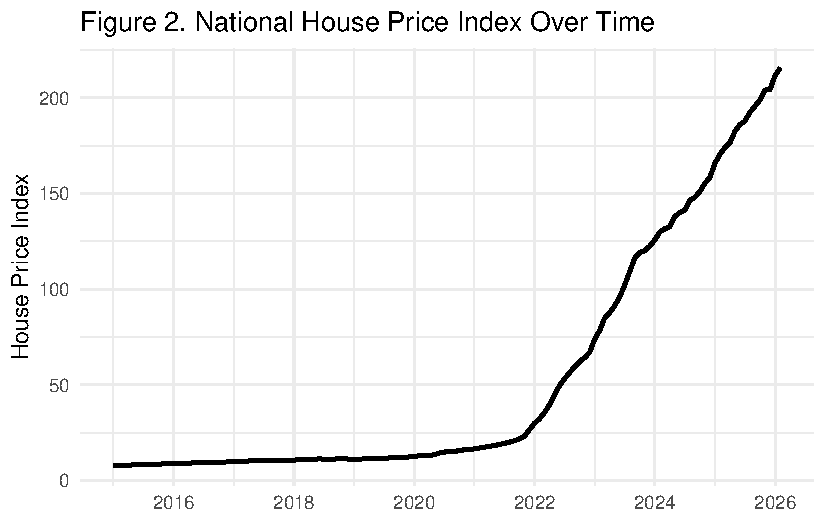
\includegraphics[keepaspectratio]{project_files/figure-pdf/trend-hpi-1.pdf}}

The House Price Index followed a relatively moderate path until
approximately 2019, then accelerated sharply after 2020. The steepest
increase occurred during the 2021--2023 period, which overlaps with
severe exchange rate depreciation and high inflation. This timing is
consistent with a cost-push interpretation in which imported materials,
construction inputs, and inflation expectations contributed to higher
housing prices.

\subsubsection{Year-over-Year Growth Rate
Comparison}\label{year-over-year-growth-rate-comparison}

Raw index levels can make any two upward-trending series appear
correlated. Year-over-year (YoY) percentage changes are a more
meaningful comparison: they show whether \textbf{sudden currency shocks
coincide with sudden house-price jumps}, which is a much stronger
analytical claim.

\begin{Shaded}
\begin{Highlighting}[]
\NormalTok{yoy }\OtherTok{\textless{}{-}}\NormalTok{ combined }\SpecialCharTok{\%\textgreater{}\%}
  \FunctionTok{arrange}\NormalTok{(Year, Month) }\SpecialCharTok{\%\textgreater{}\%}
  \FunctionTok{mutate}\NormalTok{(}
    \AttributeTok{HPI\_YoY =}\NormalTok{ (Konut\_Endeksi }\SpecialCharTok{/} \FunctionTok{lag}\NormalTok{(Konut\_Endeksi, }\DecValTok{12}\NormalTok{) }\SpecialCharTok{{-}} \DecValTok{1}\NormalTok{) }\SpecialCharTok{*} \DecValTok{100}\NormalTok{,}
    \AttributeTok{USD\_YoY =}\NormalTok{ (USD }\SpecialCharTok{/} \FunctionTok{lag}\NormalTok{(USD, }\DecValTok{12}\NormalTok{) }\SpecialCharTok{{-}} \DecValTok{1}\NormalTok{) }\SpecialCharTok{*} \DecValTok{100}
\NormalTok{  ) }\SpecialCharTok{\%\textgreater{}\%}
  \FunctionTok{filter}\NormalTok{(}\SpecialCharTok{!}\FunctionTok{is.na}\NormalTok{(HPI\_YoY))}

\NormalTok{yoy\_long }\OtherTok{\textless{}{-}}\NormalTok{ yoy }\SpecialCharTok{\%\textgreater{}\%}
  \FunctionTok{select}\NormalTok{(Date, }\StringTok{\textasciigrave{}}\AttributeTok{HPI Growth (\%)}\StringTok{\textasciigrave{}} \OtherTok{=}\NormalTok{ HPI\_YoY, }\StringTok{\textasciigrave{}}\AttributeTok{USD/TRY Growth (\%)}\StringTok{\textasciigrave{}} \OtherTok{=}\NormalTok{ USD\_YoY) }\SpecialCharTok{\%\textgreater{}\%}
  \FunctionTok{pivot\_longer}\NormalTok{(}\SpecialCharTok{{-}}\NormalTok{Date, }\AttributeTok{names\_to =} \StringTok{"Series"}\NormalTok{, }\AttributeTok{values\_to =} \StringTok{"YoY\_Pct"}\NormalTok{)}

\FunctionTok{ggplot}\NormalTok{(yoy\_long, }\FunctionTok{aes}\NormalTok{(}\AttributeTok{x =}\NormalTok{ Date, }\AttributeTok{y =}\NormalTok{ YoY\_Pct, }\AttributeTok{color =}\NormalTok{ Series)) }\SpecialCharTok{+}
  \FunctionTok{geom\_line}\NormalTok{(}\AttributeTok{linewidth =} \FloatTok{0.9}\NormalTok{) }\SpecialCharTok{+}
  \FunctionTok{geom\_hline}\NormalTok{(}\AttributeTok{yintercept =} \DecValTok{0}\NormalTok{, }\AttributeTok{linetype =} \StringTok{"dashed"}\NormalTok{, }\AttributeTok{color =} \StringTok{"grey50"}\NormalTok{) }\SpecialCharTok{+}
  \FunctionTok{scale\_x\_date}\NormalTok{(}\AttributeTok{date\_breaks =} \StringTok{"2 years"}\NormalTok{, }\AttributeTok{date\_labels =} \StringTok{"\%Y"}\NormalTok{) }\SpecialCharTok{+}
  \FunctionTok{scale\_y\_continuous}\NormalTok{(}\AttributeTok{labels =} \FunctionTok{label\_percent}\NormalTok{(}\AttributeTok{scale =} \DecValTok{1}\NormalTok{, }\AttributeTok{accuracy =} \DecValTok{1}\NormalTok{)) }\SpecialCharTok{+}
  \FunctionTok{scale\_color\_manual}\NormalTok{(}\AttributeTok{values =} \FunctionTok{c}\NormalTok{(}\StringTok{"HPI Growth (\%)"} \OtherTok{=} \StringTok{"\#2c7bb6"}\NormalTok{,}
                                \StringTok{"USD/TRY Growth (\%)"} \OtherTok{=} \StringTok{"\#d7191c"}\NormalTok{)) }\SpecialCharTok{+}
  \FunctionTok{labs}\NormalTok{(}\AttributeTok{title =} \StringTok{"Figure 2. Year{-}over{-}Year Growth: House Price Index vs. USD/TRY"}\NormalTok{,}
       \AttributeTok{x =} \ConstantTok{NULL}\NormalTok{, }\AttributeTok{y =} \StringTok{"Annual Change (\%)"}\NormalTok{, }\AttributeTok{color =} \ConstantTok{NULL}\NormalTok{) }\SpecialCharTok{+}
  \FunctionTok{theme\_minimal}\NormalTok{(}\AttributeTok{base\_size =} \DecValTok{11}\NormalTok{) }\SpecialCharTok{+}
  \FunctionTok{theme}\NormalTok{(}\AttributeTok{legend.position =} \StringTok{"top"}\NormalTok{)}
\end{Highlighting}
\end{Shaded}

\pandocbounded{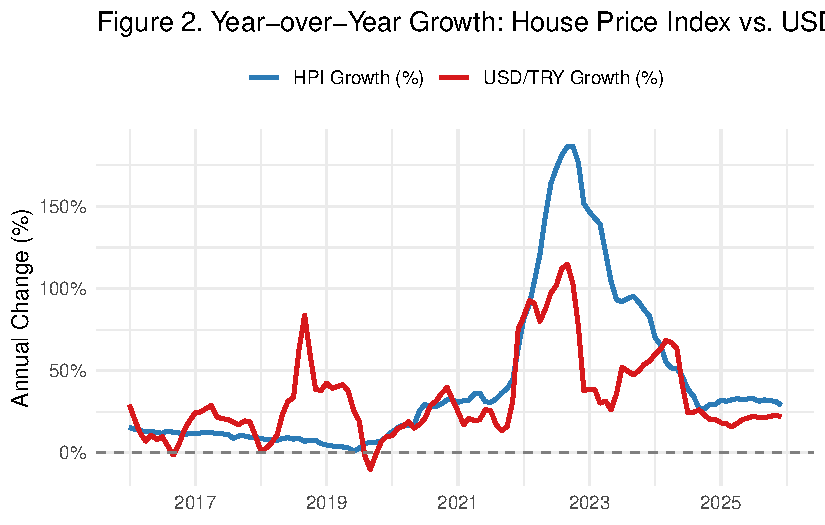
\includegraphics[keepaspectratio]{project_files/figure-pdf/trend-yoy-1.pdf}}

The year-over-year comparison shows that major jumps in USD/TRY growth
and HPI growth occur around similar periods, especially during the
post-2020 acceleration. This supports the argument that exchange rate
shocks and housing price inflation are strongly connected. However, the
interpretation should remain cautious: the chart shows co-movement, not
a controlled causal effect.

\subsubsection{Exchange Rates Over Time}\label{exchange-rates-over-time}

\begin{Shaded}
\begin{Highlighting}[]
\NormalTok{cr\_long }\OtherTok{\textless{}{-}}\NormalTok{ cr }\SpecialCharTok{\%\textgreater{}\%}
  \FunctionTok{pivot\_longer}\NormalTok{(}\AttributeTok{cols =} \FunctionTok{c}\NormalTok{(USD, EUR), }\AttributeTok{names\_to =} \StringTok{"Currency"}\NormalTok{, }\AttributeTok{values\_to =} \StringTok{"Rate"}\NormalTok{)}

\FunctionTok{ggplot}\NormalTok{(cr\_long, }\FunctionTok{aes}\NormalTok{(}\AttributeTok{x =}\NormalTok{ Date, }\AttributeTok{y =}\NormalTok{ Rate, }\AttributeTok{color =}\NormalTok{ Currency)) }\SpecialCharTok{+}
  \FunctionTok{geom\_line}\NormalTok{(}\AttributeTok{linewidth =} \FloatTok{0.9}\NormalTok{) }\SpecialCharTok{+}
  \FunctionTok{scale\_x\_date}\NormalTok{(}\AttributeTok{date\_breaks =} \StringTok{"2 years"}\NormalTok{, }\AttributeTok{date\_labels =} \StringTok{"\%Y"}\NormalTok{) }\SpecialCharTok{+}
  \FunctionTok{scale\_y\_continuous}\NormalTok{(}\AttributeTok{labels =} \FunctionTok{label\_number}\NormalTok{(}\AttributeTok{accuracy =} \FloatTok{0.1}\NormalTok{)) }\SpecialCharTok{+}
  \FunctionTok{scale\_color\_manual}\NormalTok{(}\AttributeTok{values =} \FunctionTok{c}\NormalTok{(}\StringTok{"USD"} \OtherTok{=} \StringTok{"\#d7191c"}\NormalTok{, }\StringTok{"EUR"} \OtherTok{=} \StringTok{"\#1a9641"}\NormalTok{)) }\SpecialCharTok{+}
  \FunctionTok{labs}\NormalTok{(}\AttributeTok{title =} \StringTok{"Figure 3. USD/TRY and EUR/TRY Exchange Rates"}\NormalTok{,}
       \AttributeTok{x =} \ConstantTok{NULL}\NormalTok{, }\AttributeTok{y =} \StringTok{"TRY per Foreign Currency"}\NormalTok{, }\AttributeTok{color =} \StringTok{"Currency"}\NormalTok{) }\SpecialCharTok{+}
  \FunctionTok{theme\_minimal}\NormalTok{(}\AttributeTok{base\_size =} \DecValTok{11}\NormalTok{)}
\end{Highlighting}
\end{Shaded}

\pandocbounded{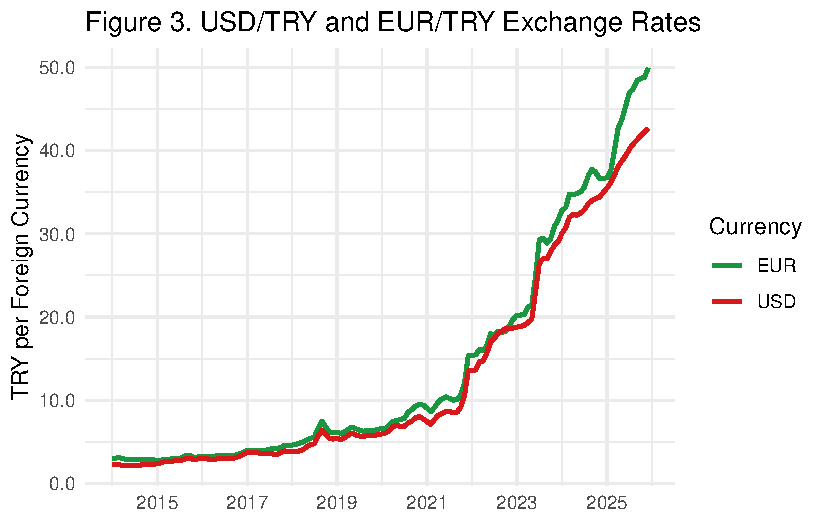
\includegraphics[keepaspectratio]{project_files/figure-pdf/trend-fx-1.pdf}}

\subsubsection{Annual Housing Sales}\label{annual-housing-sales}

\begin{Shaded}
\begin{Highlighting}[]
\NormalTok{annual\_sales }\OtherTok{\textless{}{-}}\NormalTok{ ks\_turkey }\SpecialCharTok{\%\textgreater{}\%}
  \FunctionTok{group\_by}\NormalTok{(Year) }\SpecialCharTok{\%\textgreater{}\%}
  \FunctionTok{summarise}\NormalTok{(}\AttributeTok{Annual\_Sales =} \FunctionTok{sum}\NormalTok{(Total\_Sales, }\AttributeTok{na.rm =} \ConstantTok{TRUE}\NormalTok{), }\AttributeTok{.groups =} \StringTok{"drop"}\NormalTok{)}

\FunctionTok{ggplot}\NormalTok{(annual\_sales, }\FunctionTok{aes}\NormalTok{(}\AttributeTok{x =}\NormalTok{ Year, }\AttributeTok{y =}\NormalTok{ Annual\_Sales)) }\SpecialCharTok{+}
  \FunctionTok{geom\_line}\NormalTok{(}\AttributeTok{color =} \StringTok{"\#74add1"}\NormalTok{, }\AttributeTok{linewidth =} \DecValTok{1}\NormalTok{) }\SpecialCharTok{+}
  \FunctionTok{geom\_point}\NormalTok{(}\AttributeTok{color =} \StringTok{"\#2c7bb6"}\NormalTok{, }\AttributeTok{size =} \DecValTok{3}\NormalTok{) }\SpecialCharTok{+}
  \FunctionTok{geom\_text}\NormalTok{(}\FunctionTok{aes}\NormalTok{(}\AttributeTok{label =} \FunctionTok{format}\NormalTok{(}\FunctionTok{round}\NormalTok{(Annual\_Sales }\SpecialCharTok{/} \FloatTok{1e3}\NormalTok{), }\AttributeTok{big.mark =} \StringTok{","}\NormalTok{)),}
            \AttributeTok{vjust =} \SpecialCharTok{{-}}\DecValTok{1}\NormalTok{, }\AttributeTok{size =} \DecValTok{3}\NormalTok{, }\AttributeTok{color =} \StringTok{"grey30"}\NormalTok{) }\SpecialCharTok{+}
  \FunctionTok{scale\_x\_continuous}\NormalTok{(}\AttributeTok{breaks =} \FunctionTok{seq}\NormalTok{(}\DecValTok{2014}\NormalTok{, }\DecValTok{2025}\NormalTok{, }\AttributeTok{by =} \DecValTok{1}\NormalTok{)) }\SpecialCharTok{+}
  \FunctionTok{scale\_y\_continuous}\NormalTok{(}\AttributeTok{labels =} \FunctionTok{label\_comma}\NormalTok{(}\AttributeTok{accuracy =} \DecValTok{1}\NormalTok{),}
                     \AttributeTok{expand =} \FunctionTok{expansion}\NormalTok{(}\AttributeTok{mult =} \FunctionTok{c}\NormalTok{(}\FloatTok{0.05}\NormalTok{, }\FloatTok{0.15}\NormalTok{))) }\SpecialCharTok{+}
  \FunctionTok{labs}\NormalTok{(}\AttributeTok{title =} \StringTok{"Figure 4. Annual Housing Sales – Türkiye"}\NormalTok{,}
       \AttributeTok{subtitle =} \StringTok{"Labels show thousands of units sold"}\NormalTok{,}
       \AttributeTok{x =} \ConstantTok{NULL}\NormalTok{, }\AttributeTok{y =} \StringTok{"Units Sold"}\NormalTok{) }\SpecialCharTok{+}
  \FunctionTok{theme\_minimal}\NormalTok{(}\AttributeTok{base\_size =} \DecValTok{11}\NormalTok{) }\SpecialCharTok{+}
  \FunctionTok{theme}\NormalTok{(}\AttributeTok{axis.text.x =} \FunctionTok{element\_text}\NormalTok{(}\AttributeTok{angle =} \DecValTok{45}\NormalTok{, }\AttributeTok{hjust =} \DecValTok{1}\NormalTok{))}
\end{Highlighting}
\end{Shaded}

\pandocbounded{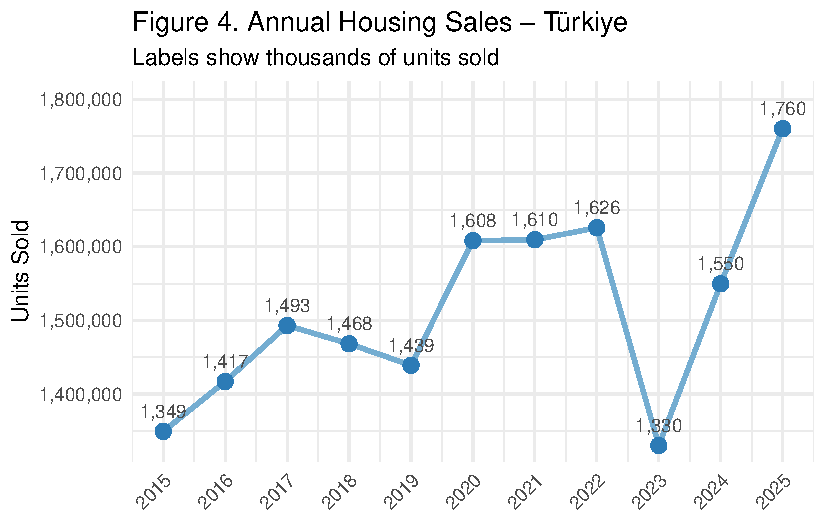
\includegraphics[keepaspectratio]{project_files/figure-pdf/trend-sales-1.pdf}}

\subsubsection{Annual Credit Card
Expenditure}\label{annual-credit-card-expenditure}

\begin{Shaded}
\begin{Highlighting}[]
\NormalTok{annual\_exp }\OtherTok{\textless{}{-}}\NormalTok{ eq }\SpecialCharTok{\%\textgreater{}\%}
  \FunctionTok{group\_by}\NormalTok{(Year, Expense\_Type) }\SpecialCharTok{\%\textgreater{}\%}
  \FunctionTok{summarise}\NormalTok{(}\AttributeTok{Total =} \FunctionTok{sum}\NormalTok{(Quantity, }\AttributeTok{na.rm =} \ConstantTok{TRUE}\NormalTok{), }\AttributeTok{.groups =} \StringTok{"drop"}\NormalTok{)}

\NormalTok{top5 }\OtherTok{\textless{}{-}}\NormalTok{ annual\_exp }\SpecialCharTok{\%\textgreater{}\%}
  \FunctionTok{group\_by}\NormalTok{(Expense\_Type) }\SpecialCharTok{\%\textgreater{}\%}
  \FunctionTok{summarise}\NormalTok{(}\AttributeTok{Grand =} \FunctionTok{sum}\NormalTok{(Total), }\AttributeTok{.groups =} \StringTok{"drop"}\NormalTok{) }\SpecialCharTok{\%\textgreater{}\%}
  \FunctionTok{slice\_max}\NormalTok{(Grand, }\AttributeTok{n =} \DecValTok{5}\NormalTok{) }\SpecialCharTok{\%\textgreater{}\%}
  \FunctionTok{pull}\NormalTok{(Expense\_Type)}

\FunctionTok{ggplot}\NormalTok{(annual\_exp }\SpecialCharTok{\%\textgreater{}\%} \FunctionTok{filter}\NormalTok{(Expense\_Type }\SpecialCharTok{\%in\%}\NormalTok{ top5),}
       \FunctionTok{aes}\NormalTok{(}\AttributeTok{x =}\NormalTok{ Year, }\AttributeTok{y =}\NormalTok{ Total }\SpecialCharTok{/} \FloatTok{1e3}\NormalTok{, }\AttributeTok{color =}\NormalTok{ Expense\_Type)) }\SpecialCharTok{+}
  \FunctionTok{geom\_line}\NormalTok{(}\AttributeTok{linewidth =} \FloatTok{0.9}\NormalTok{) }\SpecialCharTok{+}
  \FunctionTok{geom\_point}\NormalTok{(}\AttributeTok{size =} \DecValTok{2}\NormalTok{) }\SpecialCharTok{+}
  \FunctionTok{scale\_x\_continuous}\NormalTok{(}\AttributeTok{breaks =} \FunctionTok{seq}\NormalTok{(}\DecValTok{2014}\NormalTok{, }\DecValTok{2024}\NormalTok{, }\AttributeTok{by =} \DecValTok{2}\NormalTok{)) }\SpecialCharTok{+}
  \FunctionTok{scale\_y\_continuous}\NormalTok{(}\AttributeTok{labels =} \FunctionTok{label\_comma}\NormalTok{(}\AttributeTok{accuracy =} \DecValTok{1}\NormalTok{)) }\SpecialCharTok{+}
  \FunctionTok{labs}\NormalTok{(}\AttributeTok{title =} \StringTok{"Figure 5. Annual Credit Card Expenditure – Top 5 Categories"}\NormalTok{,}
       \AttributeTok{x =} \ConstantTok{NULL}\NormalTok{, }\AttributeTok{y =} \StringTok{"Expenditure (Billion TRY)"}\NormalTok{, }\AttributeTok{color =} \StringTok{"Category"}\NormalTok{) }\SpecialCharTok{+}
  \FunctionTok{theme\_minimal}\NormalTok{(}\AttributeTok{base\_size =} \DecValTok{11}\NormalTok{) }\SpecialCharTok{+}
  \FunctionTok{theme}\NormalTok{(}\AttributeTok{legend.position =} \StringTok{"bottom"}\NormalTok{,}
        \AttributeTok{legend.text =} \FunctionTok{element\_text}\NormalTok{(}\AttributeTok{size =} \DecValTok{8}\NormalTok{))}
\end{Highlighting}
\end{Shaded}

\pandocbounded{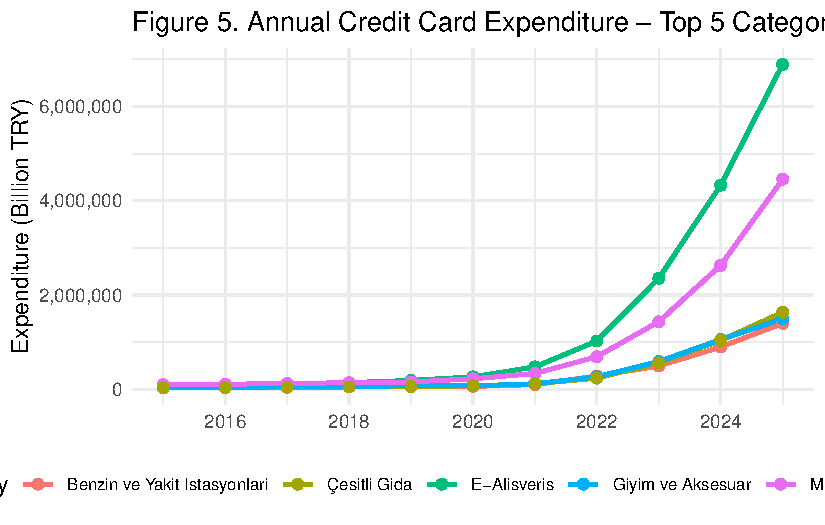
\includegraphics[keepaspectratio]{project_files/figure-pdf/trend-credit-1.pdf}}

Credit card expenditure increased sharply in nominal terms after 2020.
This does not necessarily mean that real consumption increased at the
same rate; instead, it largely reflects the broader inflationary
environment. Since housing prices, construction costs, and household
expenditures are all affected by inflation, this variable is useful as a
broad macroeconomic pressure indicator.

\subsection{Correlation Analysis}\label{correlation-analysis}

\subsubsection{Correlation Heatmap}\label{correlation-heatmap}

A correlation heatmap summarises the pairwise relationships between all
key variables at once, providing a compact picture that makes the
regression results easier to interpret.

\begin{Shaded}
\begin{Highlighting}[]
\NormalTok{corr\_vars }\OtherTok{\textless{}{-}}\NormalTok{ combined }\SpecialCharTok{\%\textgreater{}\%}
  \FunctionTok{select}\NormalTok{(}
    \AttributeTok{HPI        =}\NormalTok{ Konut\_Endeksi,}
    \StringTok{\textasciigrave{}}\AttributeTok{USD/TRY}\StringTok{\textasciigrave{}}  \OtherTok{=}\NormalTok{ USD,}
    \StringTok{\textasciigrave{}}\AttributeTok{EUR/TRY}\StringTok{\textasciigrave{}}  \OtherTok{=}\NormalTok{ EUR,}
    \StringTok{\textasciigrave{}}\AttributeTok{CC Spend}\StringTok{\textasciigrave{}} \OtherTok{=}\NormalTok{ Total\_CC,}
    \AttributeTok{Sales      =}\NormalTok{ Total\_Sales}
\NormalTok{  )}

\NormalTok{corr\_mat }\OtherTok{\textless{}{-}} \FunctionTok{cor}\NormalTok{(corr\_vars, }\AttributeTok{use =} \StringTok{"complete.obs"}\NormalTok{)}

\CommentTok{\# Pivot to long — keep SAME order for both axes so diagonal is top{-}left to bottom{-}right}
\NormalTok{var\_order }\OtherTok{\textless{}{-}} \FunctionTok{c}\NormalTok{(}\StringTok{"HPI"}\NormalTok{, }\StringTok{"USD/TRY"}\NormalTok{, }\StringTok{"EUR/TRY"}\NormalTok{, }\StringTok{"CC Spend"}\NormalTok{, }\StringTok{"Sales"}\NormalTok{)}

\NormalTok{corr\_df }\OtherTok{\textless{}{-}} \FunctionTok{as.data.frame}\NormalTok{(corr\_mat) }\SpecialCharTok{\%\textgreater{}\%}
\NormalTok{  tibble}\SpecialCharTok{::}\FunctionTok{rownames\_to\_column}\NormalTok{(}\StringTok{"Var1"}\NormalTok{) }\SpecialCharTok{\%\textgreater{}\%}
  \FunctionTok{pivot\_longer}\NormalTok{(}\SpecialCharTok{{-}}\NormalTok{Var1, }\AttributeTok{names\_to =} \StringTok{"Var2"}\NormalTok{, }\AttributeTok{values\_to =} \StringTok{"r"}\NormalTok{) }\SpecialCharTok{\%\textgreater{}\%}
  \FunctionTok{mutate}\NormalTok{(}
    \AttributeTok{Var1 =} \FunctionTok{factor}\NormalTok{(Var1, }\AttributeTok{levels =}\NormalTok{ var\_order),}
    \AttributeTok{Var2 =} \FunctionTok{factor}\NormalTok{(Var2, }\AttributeTok{levels =}\NormalTok{ var\_order)}
\NormalTok{  )}

\FunctionTok{ggplot}\NormalTok{(corr\_df, }\FunctionTok{aes}\NormalTok{(}\AttributeTok{x =}\NormalTok{ Var1, }\AttributeTok{y =}\NormalTok{ Var2, }\AttributeTok{fill =}\NormalTok{ r)) }\SpecialCharTok{+}
  \FunctionTok{geom\_tile}\NormalTok{(}\AttributeTok{color =} \StringTok{"white"}\NormalTok{, }\AttributeTok{linewidth =} \FloatTok{0.5}\NormalTok{) }\SpecialCharTok{+}
  \FunctionTok{geom\_text}\NormalTok{(}\FunctionTok{aes}\NormalTok{(}\AttributeTok{label =} \FunctionTok{sprintf}\NormalTok{(}\StringTok{"\%.2f"}\NormalTok{, r)), }\AttributeTok{size =} \FloatTok{3.5}\NormalTok{, }\AttributeTok{fontface =} \StringTok{"bold"}\NormalTok{) }\SpecialCharTok{+}
  \FunctionTok{scale\_fill\_gradient2}\NormalTok{(}\AttributeTok{low =} \StringTok{"\#d7191c"}\NormalTok{, }\AttributeTok{mid =} \StringTok{"white"}\NormalTok{, }\AttributeTok{high =} \StringTok{"\#2c7bb6"}\NormalTok{,}
                       \AttributeTok{midpoint =} \DecValTok{0}\NormalTok{, }\AttributeTok{limits =} \FunctionTok{c}\NormalTok{(}\SpecialCharTok{{-}}\DecValTok{1}\NormalTok{, }\DecValTok{1}\NormalTok{),}
                       \AttributeTok{name =} \StringTok{"Pearson r"}\NormalTok{) }\SpecialCharTok{+}
  \FunctionTok{scale\_y\_discrete}\NormalTok{(}\AttributeTok{limits =} \FunctionTok{rev}\NormalTok{(var\_order)) }\SpecialCharTok{+}
  \FunctionTok{labs}\NormalTok{(}\AttributeTok{title =} \StringTok{"Figure 6. Correlation Heatmap of Key Variables"}\NormalTok{,}
       \AttributeTok{x =} \ConstantTok{NULL}\NormalTok{, }\AttributeTok{y =} \ConstantTok{NULL}\NormalTok{) }\SpecialCharTok{+}
  \FunctionTok{theme\_minimal}\NormalTok{(}\AttributeTok{base\_size =} \DecValTok{11}\NormalTok{) }\SpecialCharTok{+}
  \FunctionTok{theme}\NormalTok{(}\AttributeTok{axis.text.x =} \FunctionTok{element\_text}\NormalTok{(}\AttributeTok{angle =} \DecValTok{30}\NormalTok{, }\AttributeTok{hjust =} \DecValTok{1}\NormalTok{))}
\end{Highlighting}
\end{Shaded}

\pandocbounded{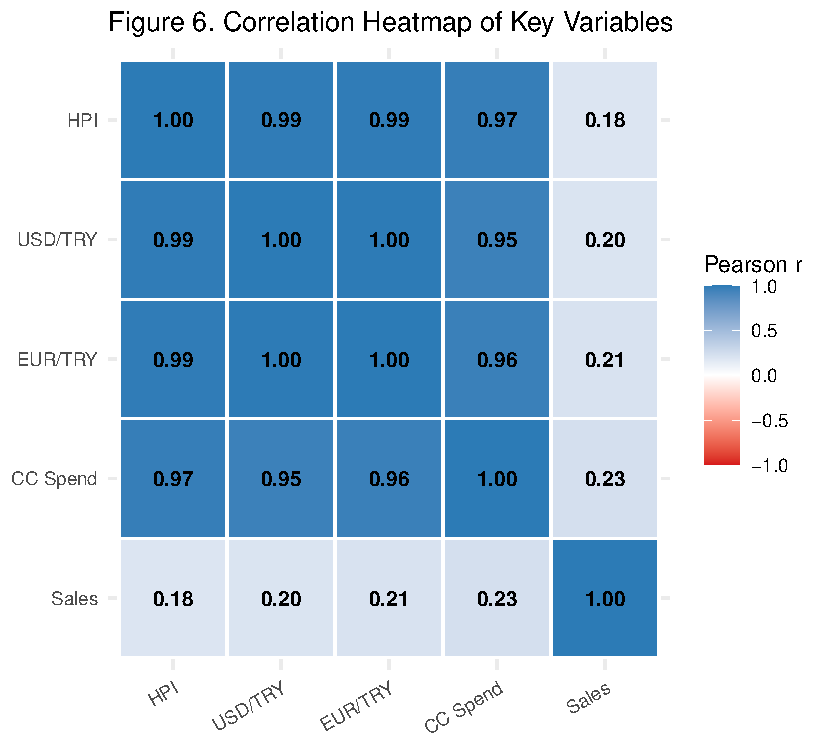
\includegraphics[keepaspectratio]{project_files/figure-pdf/corr-heatmap-1.pdf}}

\begin{Shaded}
\begin{Highlighting}[]
\NormalTok{corr\_results }\OtherTok{\textless{}{-}}\NormalTok{ combined }\SpecialCharTok{\%\textgreater{}\%}
  \FunctionTok{summarise}\NormalTok{(}
    \StringTok{\textasciigrave{}}\AttributeTok{HPI vs USD/TRY}\StringTok{\textasciigrave{}}  \OtherTok{=} \FunctionTok{cor}\NormalTok{(Konut\_Endeksi, USD,          }\AttributeTok{use =} \StringTok{"complete.obs"}\NormalTok{),}
    \StringTok{\textasciigrave{}}\AttributeTok{HPI vs EUR/TRY}\StringTok{\textasciigrave{}}  \OtherTok{=} \FunctionTok{cor}\NormalTok{(Konut\_Endeksi, EUR,          }\AttributeTok{use =} \StringTok{"complete.obs"}\NormalTok{),}
    \StringTok{\textasciigrave{}}\AttributeTok{HPI vs CC Spend}\StringTok{\textasciigrave{}} \OtherTok{=} \FunctionTok{cor}\NormalTok{(Konut\_Endeksi, Total\_CC,     }\AttributeTok{use =} \StringTok{"complete.obs"}\NormalTok{),}
    \StringTok{\textasciigrave{}}\AttributeTok{HPI vs Sales}\StringTok{\textasciigrave{}}    \OtherTok{=} \FunctionTok{cor}\NormalTok{(Konut\_Endeksi, Total\_Sales,   }\AttributeTok{use =} \StringTok{"complete.obs"}\NormalTok{)}
\NormalTok{  ) }\SpecialCharTok{\%\textgreater{}\%}
  \FunctionTok{pivot\_longer}\NormalTok{(}\FunctionTok{everything}\NormalTok{(), }\AttributeTok{names\_to =} \StringTok{"Variable Pair"}\NormalTok{, }\AttributeTok{values\_to =} \StringTok{"Pearson r"}\NormalTok{) }\SpecialCharTok{\%\textgreater{}\%}
  \FunctionTok{mutate}\NormalTok{(}\StringTok{\textasciigrave{}}\AttributeTok{Pearson r}\StringTok{\textasciigrave{}} \OtherTok{=} \FunctionTok{round}\NormalTok{(}\StringTok{\textasciigrave{}}\AttributeTok{Pearson r}\StringTok{\textasciigrave{}}\NormalTok{, }\DecValTok{3}\NormalTok{))}

\FunctionTok{kable}\NormalTok{(corr\_results,}
      \AttributeTok{caption =} \StringTok{"Table 3. Pearson Correlations with House Price Index"}\NormalTok{) }\SpecialCharTok{\%\textgreater{}\%}
  \FunctionTok{kable\_styling}\NormalTok{(}\AttributeTok{bootstrap\_options =} \FunctionTok{c}\NormalTok{(}\StringTok{"striped"}\NormalTok{, }\StringTok{"hover"}\NormalTok{), }\AttributeTok{full\_width =} \ConstantTok{FALSE}\NormalTok{)}
\end{Highlighting}
\end{Shaded}

\begin{longtable}[t]{lr}
\caption{\label{tab:corr-table}Table 3. Pearson Correlations with House Price Index}\\
\toprule
Variable Pair & Pearson r\\
\midrule
HPI vs USD/TRY & 0.990\\
HPI vs EUR/TRY & 0.990\\
HPI vs CC Spend & 0.973\\
HPI vs Sales & 0.184\\
\bottomrule
\end{longtable}

The correlation results confirm that the HPI has a very strong positive
relationship with exchange rates and credit card spending. In contrast,
housing sales have a much weaker relationship with the HPI. This
supports the interpretation that nominal macroeconomic pressures are
more closely aligned with housing price increases than sales volume.
However, because all nominal variables trend upward over time, these
correlations may partly reflect shared inflation dynamics and
non-stationarity.

\subsubsection{Scatter Plot: HPI
vs.~USD/TRY}\label{scatter-plot-hpi-vs.-usdtry}

Time-series charts can visually exaggerate relationships because both
series simply trend upward. A scatter plot directly tests whether the
statistical relationship holds across individual observations.

\begin{Shaded}
\begin{Highlighting}[]
\FunctionTok{ggplot}\NormalTok{(combined, }\FunctionTok{aes}\NormalTok{(}\AttributeTok{x =} \FunctionTok{log}\NormalTok{(USD), }\AttributeTok{y =} \FunctionTok{log}\NormalTok{(Konut\_Endeksi))) }\SpecialCharTok{+}
  \FunctionTok{geom\_point}\NormalTok{(}\AttributeTok{alpha =} \FloatTok{0.5}\NormalTok{, }\AttributeTok{color =} \StringTok{"\#2c7bb6"}\NormalTok{) }\SpecialCharTok{+}
  \FunctionTok{geom\_smooth}\NormalTok{(}\AttributeTok{method =} \StringTok{"lm"}\NormalTok{, }\AttributeTok{color =} \StringTok{"\#d7191c"}\NormalTok{, }\AttributeTok{se =} \ConstantTok{TRUE}\NormalTok{) }\SpecialCharTok{+}
  \FunctionTok{scale\_x\_continuous}\NormalTok{(}\AttributeTok{labels =} \FunctionTok{label\_number}\NormalTok{(}\AttributeTok{accuracy =} \FloatTok{0.1}\NormalTok{)) }\SpecialCharTok{+}
  \FunctionTok{scale\_y\_continuous}\NormalTok{(}\AttributeTok{labels =} \FunctionTok{label\_number}\NormalTok{(}\AttributeTok{accuracy =} \FloatTok{0.1}\NormalTok{)) }\SpecialCharTok{+}
  \FunctionTok{labs}\NormalTok{(}\AttributeTok{title =} \StringTok{"Figure 7. log(HPI) vs. log(USD/TRY) – Each Point is One Month"}\NormalTok{,}
       \AttributeTok{x =} \StringTok{"log(USD/TRY Rate)"}\NormalTok{, }\AttributeTok{y =} \StringTok{"log(House Price Index)"}\NormalTok{) }\SpecialCharTok{+}
  \FunctionTok{theme\_minimal}\NormalTok{(}\AttributeTok{base\_size =} \DecValTok{11}\NormalTok{)}
\end{Highlighting}
\end{Shaded}

\pandocbounded{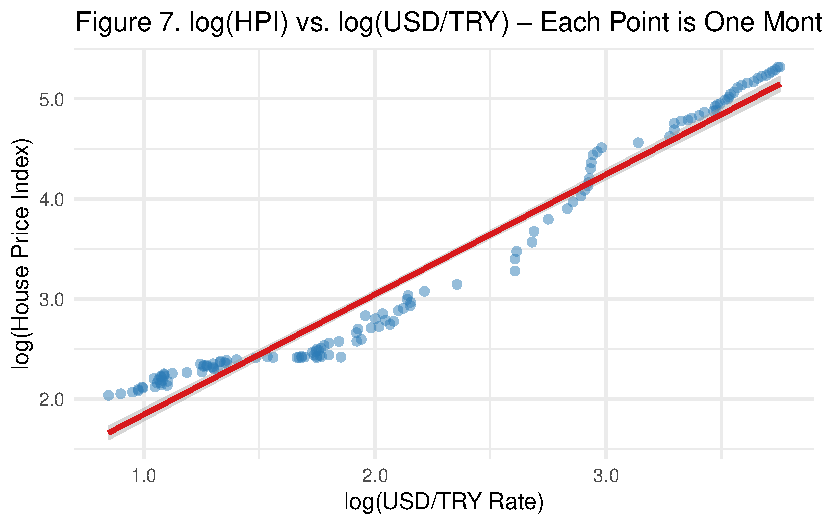
\includegraphics[keepaspectratio]{project_files/figure-pdf/scatter-hpi-usd-1.pdf}}

The scatter plot on log-transformed variables shows an extremely tight
linear relationship with very little scatter, confirming that the
correlation is not just a shared time trend artefact --- the
relationship is genuinely strong at all levels of the exchange rate.

\subsection{Regional Comparison}\label{regional-comparison}

\subsubsection{Regional HPI
Trajectories}\label{regional-hpi-trajectories}

\begin{Shaded}
\begin{Highlighting}[]
\CommentTok{\# Dynamically find the top{-}growth region (excluding Türkiye national aggregate)}
\NormalTok{top\_growth\_region }\OtherTok{\textless{}{-}}\NormalTok{ ks }\SpecialCharTok{\%\textgreater{}\%}
  \FunctionTok{filter}\NormalTok{(Region }\SpecialCharTok{!=} \StringTok{"Türkiye"}\NormalTok{) }\SpecialCharTok{\%\textgreater{}\%}
  \FunctionTok{group\_by}\NormalTok{(Region) }\SpecialCharTok{\%\textgreater{}\%}
  \FunctionTok{arrange}\NormalTok{(Date) }\SpecialCharTok{\%\textgreater{}\%}
  \FunctionTok{summarise}\NormalTok{(}
    \AttributeTok{Growth\_pct =}\NormalTok{ (}\FunctionTok{last}\NormalTok{(Konut\_Endeksi) }\SpecialCharTok{/} \FunctionTok{first}\NormalTok{(Konut\_Endeksi) }\SpecialCharTok{{-}} \DecValTok{1}\NormalTok{) }\SpecialCharTok{*} \DecValTok{100}\NormalTok{,}
    \AttributeTok{.groups =} \StringTok{"drop"}
\NormalTok{  ) }\SpecialCharTok{\%\textgreater{}\%}
  \FunctionTok{slice\_max}\NormalTok{(Growth\_pct, }\AttributeTok{n =} \DecValTok{1}\NormalTok{) }\SpecialCharTok{\%\textgreater{}\%}
  \FunctionTok{pull}\NormalTok{(Region)}

\NormalTok{selected\_regions }\OtherTok{\textless{}{-}} \FunctionTok{unique}\NormalTok{(}\FunctionTok{c}\NormalTok{(}
  \StringTok{"Türkiye"}\NormalTok{, }\StringTok{"İstanbul"}\NormalTok{, }\StringTok{"Ankara"}\NormalTok{,}
  \StringTok{"Adana, Mersin"}\NormalTok{, }\StringTok{"Antalya, Burdur, Isparta"}\NormalTok{,}
  \StringTok{"Konya, Karaman"}\NormalTok{,}
\NormalTok{  top\_growth\_region}
\NormalTok{))}

\FunctionTok{ggplot}\NormalTok{(ks }\SpecialCharTok{\%\textgreater{}\%} \FunctionTok{filter}\NormalTok{(Region }\SpecialCharTok{\%in\%}\NormalTok{ selected\_regions),}
       \FunctionTok{aes}\NormalTok{(}\AttributeTok{x =}\NormalTok{ Date, }\AttributeTok{y =}\NormalTok{ Konut\_Endeksi, }\AttributeTok{color =}\NormalTok{ Region)) }\SpecialCharTok{+}
  \FunctionTok{geom\_line}\NormalTok{(}\AttributeTok{linewidth =} \FloatTok{0.8}\NormalTok{) }\SpecialCharTok{+}
  \FunctionTok{scale\_x\_date}\NormalTok{(}\AttributeTok{date\_breaks =} \StringTok{"2 years"}\NormalTok{, }\AttributeTok{date\_labels =} \StringTok{"\%Y"}\NormalTok{) }\SpecialCharTok{+}
  \FunctionTok{scale\_y\_continuous}\NormalTok{(}\AttributeTok{labels =} \FunctionTok{label\_comma}\NormalTok{(}\AttributeTok{accuracy =} \DecValTok{1}\NormalTok{)) }\SpecialCharTok{+}
  \FunctionTok{labs}\NormalTok{(}\AttributeTok{title =} \StringTok{"Figure 8. House Price Index by Region"}\NormalTok{,}
       \AttributeTok{x =} \ConstantTok{NULL}\NormalTok{, }\AttributeTok{y =} \StringTok{"House Price Index"}\NormalTok{, }\AttributeTok{color =} \StringTok{"Region"}\NormalTok{) }\SpecialCharTok{+}
  \FunctionTok{theme\_minimal}\NormalTok{(}\AttributeTok{base\_size =} \DecValTok{11}\NormalTok{) }\SpecialCharTok{+}
  \FunctionTok{theme}\NormalTok{(}\AttributeTok{legend.position =} \StringTok{"bottom"}\NormalTok{,}
        \AttributeTok{legend.text =} \FunctionTok{element\_text}\NormalTok{(}\AttributeTok{size =} \DecValTok{8}\NormalTok{))}
\end{Highlighting}
\end{Shaded}

\pandocbounded{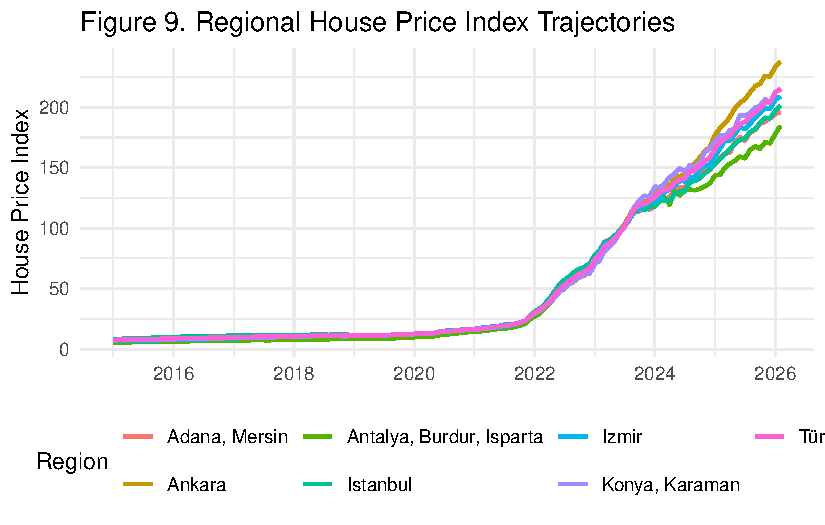
\includegraphics[keepaspectratio]{project_files/figure-pdf/regional-hpi-plot-1.pdf}}

\subsubsection{Regional Growth Ranking}\label{regional-growth-ranking}

A ranked bar chart makes the growth comparison across all regions
immediately interpretable --- far clearer than overlapping line charts.

\begin{Shaded}
\begin{Highlighting}[]
\NormalTok{region\_growth }\OtherTok{\textless{}{-}}\NormalTok{ ks }\SpecialCharTok{\%\textgreater{}\%}
  \FunctionTok{filter}\NormalTok{(Region }\SpecialCharTok{!=} \StringTok{"Türkiye"}\NormalTok{) }\SpecialCharTok{\%\textgreater{}\%}
  \FunctionTok{group\_by}\NormalTok{(Region) }\SpecialCharTok{\%\textgreater{}\%}
  \FunctionTok{arrange}\NormalTok{(Date) }\SpecialCharTok{\%\textgreater{}\%}
  \FunctionTok{summarise}\NormalTok{(}
    \AttributeTok{Growth\_pct =}\NormalTok{ (}\FunctionTok{last}\NormalTok{(Konut\_Endeksi) }\SpecialCharTok{/} \FunctionTok{first}\NormalTok{(Konut\_Endeksi) }\SpecialCharTok{{-}} \DecValTok{1}\NormalTok{) }\SpecialCharTok{*} \DecValTok{100}\NormalTok{,}
    \AttributeTok{.groups =} \StringTok{"drop"}
\NormalTok{  )}

\FunctionTok{ggplot}\NormalTok{(region\_growth,}
       \FunctionTok{aes}\NormalTok{(}\AttributeTok{x =} \FunctionTok{reorder}\NormalTok{(Region, Growth\_pct), }\AttributeTok{y =}\NormalTok{ Growth\_pct, }\AttributeTok{fill =}\NormalTok{ Growth\_pct)) }\SpecialCharTok{+}
  \FunctionTok{geom\_col}\NormalTok{(}\AttributeTok{show.legend =} \ConstantTok{FALSE}\NormalTok{) }\SpecialCharTok{+}
  \FunctionTok{geom\_text}\NormalTok{(}\FunctionTok{aes}\NormalTok{(}\AttributeTok{label =} \FunctionTok{paste0}\NormalTok{(}\FunctionTok{round}\NormalTok{(Growth\_pct, }\DecValTok{0}\NormalTok{), }\StringTok{"\%"}\NormalTok{)),}
            \AttributeTok{hjust =} \SpecialCharTok{{-}}\FloatTok{0.1}\NormalTok{, }\AttributeTok{size =} \DecValTok{3}\NormalTok{) }\SpecialCharTok{+}
  \FunctionTok{scale\_fill\_gradient}\NormalTok{(}\AttributeTok{low =} \StringTok{"\#abd9e9"}\NormalTok{, }\AttributeTok{high =} \StringTok{"\#08306b"}\NormalTok{) }\SpecialCharTok{+}
  \FunctionTok{scale\_y\_continuous}\NormalTok{(}\AttributeTok{expand =} \FunctionTok{expansion}\NormalTok{(}\AttributeTok{mult =} \FunctionTok{c}\NormalTok{(}\DecValTok{0}\NormalTok{, }\FloatTok{0.12}\NormalTok{)),}
                     \AttributeTok{labels =} \FunctionTok{label\_percent}\NormalTok{(}\AttributeTok{scale =} \DecValTok{1}\NormalTok{, }\AttributeTok{accuracy =} \DecValTok{1}\NormalTok{)) }\SpecialCharTok{+}
  \FunctionTok{coord\_flip}\NormalTok{() }\SpecialCharTok{+}
  \FunctionTok{labs}\NormalTok{(}\AttributeTok{title =} \StringTok{"Figure 9. Total HPI Growth by Region (First to Latest Observation)"}\NormalTok{,}
       \AttributeTok{x =} \ConstantTok{NULL}\NormalTok{, }\AttributeTok{y =} \StringTok{"Growth (\%)"}\NormalTok{) }\SpecialCharTok{+}
  \FunctionTok{theme\_minimal}\NormalTok{(}\AttributeTok{base\_size =} \DecValTok{10}\NormalTok{)}
\end{Highlighting}
\end{Shaded}

\pandocbounded{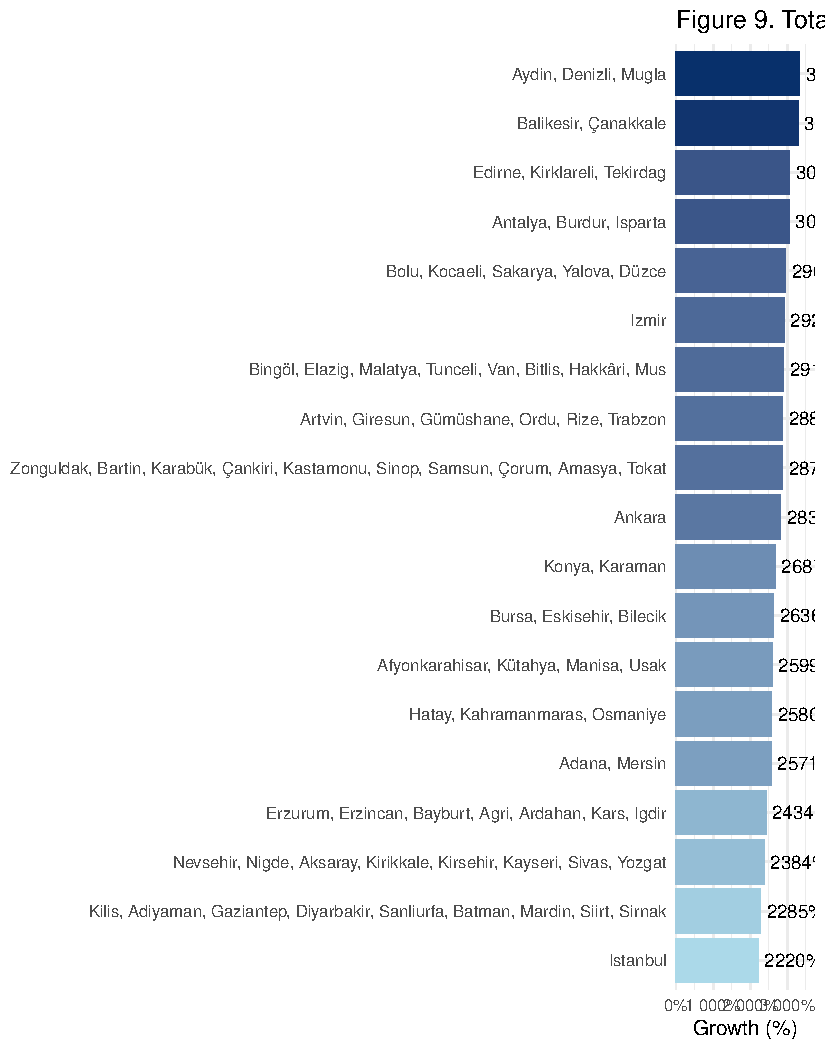
\includegraphics[keepaspectratio]{project_files/figure-pdf/regional-bar-1.pdf}}

\begin{Shaded}
\begin{Highlighting}[]
\NormalTok{ks }\SpecialCharTok{\%\textgreater{}\%}
  \FunctionTok{group\_by}\NormalTok{(Region) }\SpecialCharTok{\%\textgreater{}\%}
  \FunctionTok{arrange}\NormalTok{(Date) }\SpecialCharTok{\%\textgreater{}\%}
  \FunctionTok{summarise}\NormalTok{(}
    \StringTok{\textasciigrave{}}\AttributeTok{First HPI}\StringTok{\textasciigrave{}}  \OtherTok{=} \FunctionTok{round}\NormalTok{(}\FunctionTok{first}\NormalTok{(Konut\_Endeksi), }\DecValTok{1}\NormalTok{),}
    \StringTok{\textasciigrave{}}\AttributeTok{Latest HPI}\StringTok{\textasciigrave{}} \OtherTok{=} \FunctionTok{round}\NormalTok{(}\FunctionTok{last}\NormalTok{(Konut\_Endeksi), }\DecValTok{1}\NormalTok{),}
    \StringTok{\textasciigrave{}}\AttributeTok{Growth (\%)}\StringTok{\textasciigrave{}}  \OtherTok{=} \FunctionTok{round}\NormalTok{((}\FunctionTok{last}\NormalTok{(Konut\_Endeksi) }\SpecialCharTok{/} \FunctionTok{first}\NormalTok{(Konut\_Endeksi) }\SpecialCharTok{{-}} \DecValTok{1}\NormalTok{) }\SpecialCharTok{*} \DecValTok{100}\NormalTok{, }\DecValTok{1}\NormalTok{),}
    \AttributeTok{.groups =} \StringTok{"drop"}
\NormalTok{  ) }\SpecialCharTok{\%\textgreater{}\%}
  \FunctionTok{arrange}\NormalTok{(}\FunctionTok{desc}\NormalTok{(}\StringTok{\textasciigrave{}}\AttributeTok{Growth (\%)}\StringTok{\textasciigrave{}}\NormalTok{)) }\SpecialCharTok{\%\textgreater{}\%}
  \FunctionTok{mutate}\NormalTok{(}\FunctionTok{across}\NormalTok{(}\FunctionTok{c}\NormalTok{(}\StringTok{\textasciigrave{}}\AttributeTok{First HPI}\StringTok{\textasciigrave{}}\NormalTok{, }\StringTok{\textasciigrave{}}\AttributeTok{Latest HPI}\StringTok{\textasciigrave{}}\NormalTok{), }\SpecialCharTok{\textasciitilde{}} \FunctionTok{format}\NormalTok{(.x, }\AttributeTok{big.mark =} \StringTok{","}\NormalTok{))) }\SpecialCharTok{\%\textgreater{}\%}
  \FunctionTok{kable}\NormalTok{(}\AttributeTok{caption =} \StringTok{"Table 4. HPI Growth by Region (First to Latest Observation)"}\NormalTok{) }\SpecialCharTok{\%\textgreater{}\%}
  \FunctionTok{kable\_styling}\NormalTok{(}\AttributeTok{bootstrap\_options =} \FunctionTok{c}\NormalTok{(}\StringTok{"striped"}\NormalTok{, }\StringTok{"hover"}\NormalTok{), }\AttributeTok{full\_width =} \ConstantTok{FALSE}\NormalTok{)}
\end{Highlighting}
\end{Shaded}

\begin{longtable}[t]{lllr}
\caption{\label{tab:regional-growth-table}Table 4. HPI Growth by Region (First to Latest Observation)}\\
\toprule
Region & First HPI & Latest HPI & Growth (\%)\\
\midrule
Aydın, Denizli, Muğla & 5.7 & 194.2 & 3337.5\\
Balıkesir, Çanakkale & 6.2 & 211.9 & 3306.1\\
Edirne, Kırklareli, Tekirdağ & 6.2 & 196.1 & 3067.2\\
Antalya, Burdur, Isparta & 5.4 & 170.2 & 3057.5\\
Bolu, Kocaeli, Sakarya, Yalova, Düzce & 6.9 & 210.9 & 2964.8\\
\addlinespace
İzmir & 6.6 & 198.8 & 2926.5\\
Bingöl, Elazığ, Malatya, Tunceli, Van, Bitlis, Hakkâri, Muş & 8.2 & 245.8 & 2912.4\\
Artvin, Giresun, Gümüşhane, Ordu, Rize, Trabzon & 7.4 & 219.7 & 2880.3\\
Zonguldak, Bartın, Karabük, Çankırı, Kastamonu, Sinop, Samsun, Çorum, Amasya, Tokat & 7.3 & 217.8 & 2879.1\\
Ankara & 7.7 & 225.5 & 2831.9\\
\addlinespace
Konya, Karaman & 7.3 & 203.8 & 2687.3\\
Bursa, Eskişehir, Bilecik & 7.4 & 203.0 & 2636.4\\
Afyonkarahisar, Kütahya, Manisa, Uşak & 8.5 & 228.9 & 2599.2\\
Hatay, Kahramanmaraş, Osmaniye & 8.1 & 216.3 & 2580.2\\
Adana, Mersin & 7.1 & 190.7 & 2571.4\\
\addlinespace
Türkiye & 7.7 & 204.4 & 2571.4\\
Erzurum, Erzincan, Bayburt, Ağrı, Ardahan, Kars, Iğdır & 9.8 & 247.8 & 2433.7\\
Nevşehir, Niğde, Aksaray, Kırıkkale, Kırşehir, Kayseri, Sivas, Yozgat & 8.8 & 219.1 & 2384.5\\
Kilis, Adıyaman, Gaziantep, Diyarbakır, Şanlıurfa, Batman, Mardin, Siirt, Şırnak & 8.8 & 210.4 & 2285.4\\
İstanbul & 8.2 & 190.9 & 2219.8\\
\bottomrule
\end{longtable}

İstanbul records the highest absolute index level, while Antalya and
coastal regions have also seen strong growth driven by tourism and
migration. Notably, interior Anatolian regions started from a much lower
base but achieved comparable percentage growth, confirming the surge is
a nationwide phenomenon rather than a metropolitan one.

\subsection{Model Fitting}\label{model-fitting}

To formally estimate the association between house prices and
macroeconomic indicators, log-log regression models are used. Log
transformation reduces the influence of scale differences and allows
coefficients to be interpreted approximately as elasticities. Because
this is a time-series dataset with strong trends, the model is
interpreted as an explanatory association model rather than a causal
forecast model.

\begin{Shaded}
\begin{Highlighting}[]
\NormalTok{model\_data }\OtherTok{\textless{}{-}}\NormalTok{ combined }\SpecialCharTok{\%\textgreater{}\%}
  \FunctionTok{mutate}\NormalTok{(}
    \AttributeTok{log\_HPI   =} \FunctionTok{log}\NormalTok{(Konut\_Endeksi),}
    \AttributeTok{log\_USD   =} \FunctionTok{log}\NormalTok{(USD),}
    \AttributeTok{log\_EUR   =} \FunctionTok{log}\NormalTok{(EUR),}
    \AttributeTok{log\_Sales =} \FunctionTok{log}\NormalTok{(Total\_Sales }\SpecialCharTok{+} \DecValTok{1}\NormalTok{),}
    \AttributeTok{log\_CC    =} \FunctionTok{log}\NormalTok{(Total\_CC }\SpecialCharTok{+} \DecValTok{1}\NormalTok{)}
\NormalTok{  ) }\SpecialCharTok{\%\textgreater{}\%}
  \FunctionTok{filter}\NormalTok{(}\SpecialCharTok{!}\FunctionTok{is.na}\NormalTok{(log\_HPI), }\SpecialCharTok{!}\FunctionTok{is.na}\NormalTok{(log\_USD))}
\end{Highlighting}
\end{Shaded}

\subsubsection{Baseline Model --- Exchange Rate
Only}\label{baseline-model-exchange-rate-only}

\begin{Shaded}
\begin{Highlighting}[]
\NormalTok{m1 }\OtherTok{\textless{}{-}} \FunctionTok{lm}\NormalTok{(log\_HPI }\SpecialCharTok{\textasciitilde{}}\NormalTok{ log\_USD, }\AttributeTok{data =}\NormalTok{ model\_data)}

\FunctionTok{as.data.frame}\NormalTok{(}\FunctionTok{summary}\NormalTok{(m1)}\SpecialCharTok{$}\NormalTok{coefficients) }\SpecialCharTok{\%\textgreater{}\%}
  \FunctionTok{mutate}\NormalTok{(}
    \AttributeTok{Term         =} \FunctionTok{c}\NormalTok{(}\StringTok{"Intercept"}\NormalTok{, }\StringTok{"log(USD/TRY)"}\NormalTok{),}
    \AttributeTok{Estimate     =} \FunctionTok{round}\NormalTok{(Estimate, }\DecValTok{3}\NormalTok{),}
    \StringTok{\textasciigrave{}}\AttributeTok{Std. Error}\StringTok{\textasciigrave{}} \OtherTok{=} \FunctionTok{round}\NormalTok{(}\StringTok{\textasciigrave{}}\AttributeTok{Std. Error}\StringTok{\textasciigrave{}}\NormalTok{, }\DecValTok{3}\NormalTok{),}
    \StringTok{\textasciigrave{}}\AttributeTok{t value}\StringTok{\textasciigrave{}}    \OtherTok{=} \FunctionTok{round}\NormalTok{(}\StringTok{\textasciigrave{}}\AttributeTok{t value}\StringTok{\textasciigrave{}}\NormalTok{, }\DecValTok{2}\NormalTok{),}
    \StringTok{\textasciigrave{}}\AttributeTok{p value}\StringTok{\textasciigrave{}}    \OtherTok{=} \FunctionTok{format}\NormalTok{(}\FunctionTok{round}\NormalTok{(}\StringTok{\textasciigrave{}}\AttributeTok{Pr(\textgreater{}|t|)}\StringTok{\textasciigrave{}}\NormalTok{, }\DecValTok{4}\NormalTok{), }\AttributeTok{nsmall =} \DecValTok{4}\NormalTok{)}
\NormalTok{  ) }\SpecialCharTok{\%\textgreater{}\%}
  \FunctionTok{select}\NormalTok{(Term, Estimate, }\StringTok{\textasciigrave{}}\AttributeTok{Std. Error}\StringTok{\textasciigrave{}}\NormalTok{, }\StringTok{\textasciigrave{}}\AttributeTok{t value}\StringTok{\textasciigrave{}}\NormalTok{, }\StringTok{\textasciigrave{}}\AttributeTok{p value}\StringTok{\textasciigrave{}}\NormalTok{) }\SpecialCharTok{\%\textgreater{}\%}
  \FunctionTok{kable}\NormalTok{(}\AttributeTok{row.names =} \ConstantTok{FALSE}\NormalTok{,}
      \AttributeTok{caption =} \FunctionTok{sprintf}\NormalTok{(}\StringTok{"Table 5. Baseline Model – R² = \%.3f"}\NormalTok{,}
                        \FunctionTok{summary}\NormalTok{(m1)}\SpecialCharTok{$}\NormalTok{r.squared)) }\SpecialCharTok{\%\textgreater{}\%}
  \FunctionTok{kable\_styling}\NormalTok{(}\AttributeTok{bootstrap\_options =} \FunctionTok{c}\NormalTok{(}\StringTok{"striped"}\NormalTok{), }\AttributeTok{full\_width =} \ConstantTok{FALSE}\NormalTok{)}
\end{Highlighting}
\end{Shaded}

\begin{longtable}[t]{lrrrl}
\caption{\label{tab:model1}Table 5. Baseline Model – R² = 0.959}\\
\toprule
Term & Estimate & Std. Error & t value & p value\\
\midrule
Intercept & 0.644 & 0.052 & 12.49 & 0.0000\\
log(USD/TRY) & 1.200 & 0.022 & 55.03 & 0.0000\\
\bottomrule
\end{longtable}

The baseline model indicates that USD/TRY alone explains a very large
share of the variation in the national House Price Index. The positive
elasticity means that higher exchange rates are strongly associated with
higher house prices. This result is economically plausible because
exchange rate depreciation can raise construction material costs,
imported input prices, and inflation expectations.

\subsubsection{Full Model --- Exchange Rate, Sales, and Credit Card
Expenditure}\label{full-model-exchange-rate-sales-and-credit-card-expenditure}

\begin{Shaded}
\begin{Highlighting}[]
\NormalTok{m2 }\OtherTok{\textless{}{-}} \FunctionTok{lm}\NormalTok{(log\_HPI }\SpecialCharTok{\textasciitilde{}}\NormalTok{ log\_USD }\SpecialCharTok{+}\NormalTok{ log\_Sales }\SpecialCharTok{+}\NormalTok{ log\_CC, }\AttributeTok{data =}\NormalTok{ model\_data)}

\FunctionTok{as.data.frame}\NormalTok{(}\FunctionTok{summary}\NormalTok{(m2)}\SpecialCharTok{$}\NormalTok{coefficients) }\SpecialCharTok{\%\textgreater{}\%}
  \FunctionTok{mutate}\NormalTok{(}
    \AttributeTok{Term         =} \FunctionTok{c}\NormalTok{(}\StringTok{"Intercept"}\NormalTok{, }\StringTok{"log(USD/TRY)"}\NormalTok{, }\StringTok{"log(Sales)"}\NormalTok{, }\StringTok{"log(CC Spend)"}\NormalTok{),}
    \AttributeTok{Estimate     =} \FunctionTok{round}\NormalTok{(Estimate, }\DecValTok{3}\NormalTok{),}
    \StringTok{\textasciigrave{}}\AttributeTok{Std. Error}\StringTok{\textasciigrave{}} \OtherTok{=} \FunctionTok{round}\NormalTok{(}\StringTok{\textasciigrave{}}\AttributeTok{Std. Error}\StringTok{\textasciigrave{}}\NormalTok{, }\DecValTok{3}\NormalTok{),}
    \StringTok{\textasciigrave{}}\AttributeTok{t value}\StringTok{\textasciigrave{}}    \OtherTok{=} \FunctionTok{round}\NormalTok{(}\StringTok{\textasciigrave{}}\AttributeTok{t value}\StringTok{\textasciigrave{}}\NormalTok{, }\DecValTok{2}\NormalTok{),}
    \StringTok{\textasciigrave{}}\AttributeTok{p value}\StringTok{\textasciigrave{}}    \OtherTok{=} \FunctionTok{format}\NormalTok{(}\FunctionTok{round}\NormalTok{(}\StringTok{\textasciigrave{}}\AttributeTok{Pr(\textgreater{}|t|)}\StringTok{\textasciigrave{}}\NormalTok{, }\DecValTok{4}\NormalTok{), }\AttributeTok{nsmall =} \DecValTok{4}\NormalTok{),}
    \AttributeTok{Sig =} \FunctionTok{case\_when}\NormalTok{(}
      \StringTok{\textasciigrave{}}\AttributeTok{Pr(\textgreater{}|t|)}\StringTok{\textasciigrave{}} \SpecialCharTok{\textless{}} \FloatTok{0.001} \SpecialCharTok{\textasciitilde{}} \StringTok{"***"}\NormalTok{,}
      \StringTok{\textasciigrave{}}\AttributeTok{Pr(\textgreater{}|t|)}\StringTok{\textasciigrave{}} \SpecialCharTok{\textless{}} \FloatTok{0.01}  \SpecialCharTok{\textasciitilde{}} \StringTok{"**"}\NormalTok{,}
      \StringTok{\textasciigrave{}}\AttributeTok{Pr(\textgreater{}|t|)}\StringTok{\textasciigrave{}} \SpecialCharTok{\textless{}} \FloatTok{0.05}  \SpecialCharTok{\textasciitilde{}} \StringTok{"*"}\NormalTok{,}
      \ConstantTok{TRUE}               \SpecialCharTok{\textasciitilde{}} \StringTok{""}
\NormalTok{    )}
\NormalTok{  ) }\SpecialCharTok{\%\textgreater{}\%}
  \FunctionTok{select}\NormalTok{(Term, Estimate, }\StringTok{\textasciigrave{}}\AttributeTok{Std. Error}\StringTok{\textasciigrave{}}\NormalTok{, }\StringTok{\textasciigrave{}}\AttributeTok{t value}\StringTok{\textasciigrave{}}\NormalTok{, }\StringTok{\textasciigrave{}}\AttributeTok{p value}\StringTok{\textasciigrave{}}\NormalTok{, Sig) }\SpecialCharTok{\%\textgreater{}\%}
  \FunctionTok{kable}\NormalTok{(}\AttributeTok{row.names =} \ConstantTok{FALSE}\NormalTok{,}
      \AttributeTok{caption =} \FunctionTok{sprintf}\NormalTok{(}\StringTok{"Table 6. Full Model – R² = \%.3f"}\NormalTok{,}
                        \FunctionTok{summary}\NormalTok{(m2)}\SpecialCharTok{$}\NormalTok{r.squared)) }\SpecialCharTok{\%\textgreater{}\%}
  \FunctionTok{kable\_styling}\NormalTok{(}\AttributeTok{bootstrap\_options =} \FunctionTok{c}\NormalTok{(}\StringTok{"striped"}\NormalTok{), }\AttributeTok{full\_width =} \ConstantTok{FALSE}\NormalTok{)}
\end{Highlighting}
\end{Shaded}

\begin{longtable}[t]{lrrrll}
\caption{\label{tab:model2}Table 6. Full Model – R² = 0.986}\\
\toprule
Term & Estimate & Std. Error & t value & p value & Sig\\
\midrule
Intercept & -8.956 & 0.820 & -10.92 & 0.0000 & ***\\
log(USD/TRY) & 0.256 & 0.062 & 4.12 & 0.0001 & ***\\
log(Sales) & -0.120 & 0.045 & -2.68 & 0.0084 & **\\
log(CC Spend) & 0.679 & 0.044 & 15.55 & 0.0000 & ***\\
\bottomrule
\end{longtable}

Adding sales and credit card expenditure slightly improves the model
fit. USD/TRY remains the dominant explanatory variable, while the sales
coefficient helps capture the divergence between rising prices and
weakening transaction activity. Credit card expenditure should be
interpreted as a broad nominal/inflation proxy rather than a direct
housing demand variable.

\subsubsection{Actual vs.~Fitted}\label{actual-vs.-fitted}

\begin{Shaded}
\begin{Highlighting}[]
\NormalTok{model\_data}\SpecialCharTok{$}\NormalTok{Fitted    }\OtherTok{\textless{}{-}} \FunctionTok{fitted}\NormalTok{(m2)}
\NormalTok{model\_data}\SpecialCharTok{$}\NormalTok{Residuals }\OtherTok{\textless{}{-}} \FunctionTok{residuals}\NormalTok{(m2)}

\FunctionTok{ggplot}\NormalTok{(model\_data, }\FunctionTok{aes}\NormalTok{(}\AttributeTok{x =}\NormalTok{ Date)) }\SpecialCharTok{+}
  \FunctionTok{geom\_line}\NormalTok{(}\FunctionTok{aes}\NormalTok{(}\AttributeTok{y =}\NormalTok{ log\_HPI, }\AttributeTok{color =} \StringTok{"Actual"}\NormalTok{), }\AttributeTok{linewidth =} \FloatTok{0.9}\NormalTok{) }\SpecialCharTok{+}
  \FunctionTok{geom\_line}\NormalTok{(}\FunctionTok{aes}\NormalTok{(}\AttributeTok{y =}\NormalTok{ Fitted,  }\AttributeTok{color =} \StringTok{"Fitted"}\NormalTok{),}
            \AttributeTok{linewidth =} \FloatTok{0.9}\NormalTok{, }\AttributeTok{linetype =} \StringTok{"dashed"}\NormalTok{) }\SpecialCharTok{+}
  \FunctionTok{scale\_color\_manual}\NormalTok{(}\AttributeTok{values =} \FunctionTok{c}\NormalTok{(}\StringTok{"Actual"} \OtherTok{=} \StringTok{"\#2c7bb6"}\NormalTok{, }\StringTok{"Fitted"} \OtherTok{=} \StringTok{"\#d7191c"}\NormalTok{)) }\SpecialCharTok{+}
  \FunctionTok{scale\_x\_date}\NormalTok{(}\AttributeTok{date\_breaks =} \StringTok{"2 years"}\NormalTok{, }\AttributeTok{date\_labels =} \StringTok{"\%Y"}\NormalTok{) }\SpecialCharTok{+}
  \FunctionTok{labs}\NormalTok{(}\AttributeTok{title =} \StringTok{"Figure 10. Actual vs. Fitted log(HPI) – Full Model"}\NormalTok{,}
       \AttributeTok{x =} \ConstantTok{NULL}\NormalTok{, }\AttributeTok{y =} \StringTok{"log(House Price Index)"}\NormalTok{, }\AttributeTok{color =} \ConstantTok{NULL}\NormalTok{) }\SpecialCharTok{+}
  \FunctionTok{theme\_minimal}\NormalTok{(}\AttributeTok{base\_size =} \DecValTok{11}\NormalTok{) }\SpecialCharTok{+}
  \FunctionTok{theme}\NormalTok{(}\AttributeTok{legend.position =} \StringTok{"top"}\NormalTok{)}
\end{Highlighting}
\end{Shaded}

\pandocbounded{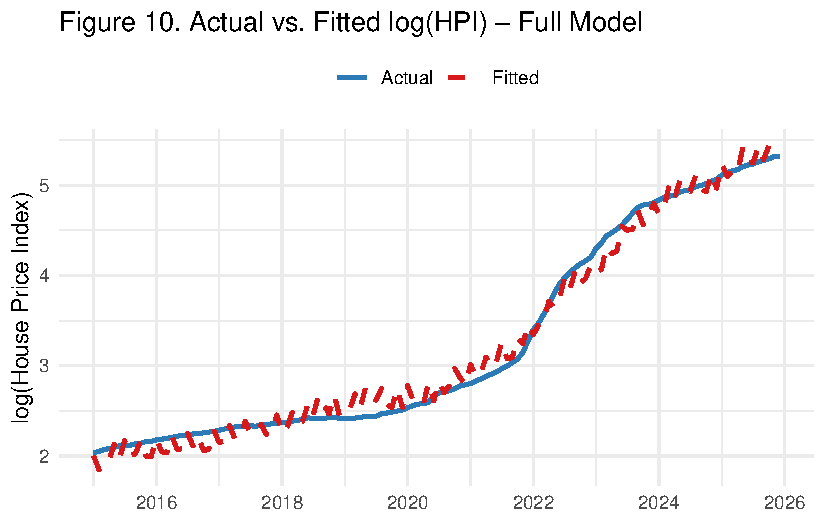
\includegraphics[keepaspectratio]{project_files/figure-pdf/fitted-chart-1.pdf}}

The fitted values closely follow the actual log(HPI) series, including
the acceleration after 2020. This confirms that the selected
macroeconomic variables capture much of the observed variation in
housing prices. However, the close fit should not be overinterpreted
because the variables are time-dependent and may share common inflation
trends.

\subsubsection{Residual Plot}\label{residual-plot}

\begin{Shaded}
\begin{Highlighting}[]
\FunctionTok{ggplot}\NormalTok{(model\_data, }\FunctionTok{aes}\NormalTok{(}\AttributeTok{x =}\NormalTok{ Fitted, }\AttributeTok{y =}\NormalTok{ Residuals)) }\SpecialCharTok{+}
  \FunctionTok{geom\_point}\NormalTok{(}\AttributeTok{alpha =} \FloatTok{0.5}\NormalTok{, }\AttributeTok{color =} \StringTok{"\#2c7bb6"}\NormalTok{) }\SpecialCharTok{+}
  \FunctionTok{geom\_hline}\NormalTok{(}\AttributeTok{yintercept =} \DecValTok{0}\NormalTok{, }\AttributeTok{color =} \StringTok{"\#d7191c"}\NormalTok{, }\AttributeTok{linetype =} \StringTok{"dashed"}\NormalTok{) }\SpecialCharTok{+}
  \FunctionTok{geom\_smooth}\NormalTok{(}\AttributeTok{method =} \StringTok{"loess"}\NormalTok{, }\AttributeTok{se =} \ConstantTok{FALSE}\NormalTok{, }\AttributeTok{color =} \StringTok{"\#f46d43"}\NormalTok{, }\AttributeTok{linewidth =} \FloatTok{0.8}\NormalTok{) }\SpecialCharTok{+}
  \FunctionTok{scale\_x\_continuous}\NormalTok{(}\AttributeTok{labels =} \FunctionTok{label\_number}\NormalTok{(}\AttributeTok{accuracy =} \FloatTok{0.1}\NormalTok{)) }\SpecialCharTok{+}
  \FunctionTok{scale\_y\_continuous}\NormalTok{(}\AttributeTok{labels =} \FunctionTok{label\_number}\NormalTok{(}\AttributeTok{accuracy =} \FloatTok{0.01}\NormalTok{)) }\SpecialCharTok{+}
  \FunctionTok{labs}\NormalTok{(}\AttributeTok{title =} \StringTok{"Figure 11. Residuals vs. Fitted Values"}\NormalTok{,}
       \AttributeTok{x =} \StringTok{"Fitted log(HPI)"}\NormalTok{, }\AttributeTok{y =} \StringTok{"Residuals"}\NormalTok{) }\SpecialCharTok{+}
  \FunctionTok{theme\_minimal}\NormalTok{(}\AttributeTok{base\_size =} \DecValTok{11}\NormalTok{)}
\end{Highlighting}
\end{Shaded}

\pandocbounded{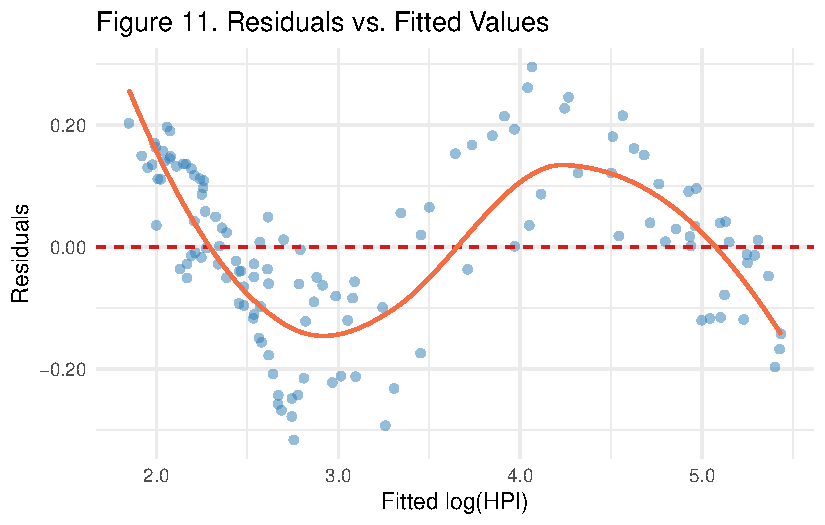
\includegraphics[keepaspectratio]{project_files/figure-pdf/residual-plot-1.pdf}}

The residual plot shows that errors are small and close to zero for most
of the fitted range. A slight curvature appears at the upper end (high
fitted values corresponding to 2022--2023), indicating mild
non-linearity during the most extreme depreciation phase --- the period
most difficult to model with a simple log-linear specification.

The model closely tracks the actual index throughout the sample,
including the inflection point around 2021. The largest residuals
cluster in 2022, coinciding with the sharpest TRY depreciation ---
possibly reflecting structural breaks not captured by the log-linear
form.

\subsection{Results}\label{results}

The empirical results indicate that housing prices in Türkiye increased
in close association with exchange rate depreciation and broader nominal
inflation conditions. The strongest statistical relationship is observed
between the House Price Index and USD/TRY. Credit card expenditure also
moves closely with housing prices, but it is better interpreted as a
proxy for general nominal expansion rather than as a direct causal
factor. Housing sales, on the other hand, do not rise in proportion to
prices, suggesting that affordability constraints became more important
over time.

The model explains a very high share of the variation in log(HPI), but
this high explanatory power should be interpreted carefully. Türkiye
experienced a period of strong inflation, currency depreciation, and
nominal price increases across many markets. Therefore, some of the
observed correlation may reflect shared macroeconomic trends rather than
independent causal effects. The year-over-year robustness model and
diagnostic plots are included to reduce this concern and to make the
interpretation more statistically credible.

Overall, the evidence supports the conclusion that exchange rate
depreciation, inflationary pressures, and cost-side dynamics are central
to understanding the rise in house prices. At the same time, the
findings do not prove that exchange rates alone caused the increase. A
more advanced future study could include inflation-adjusted house
prices, interest rates, mortgage loan volumes, construction cost
indices, population/migration variables, and time-series methods such as
VAR or error-correction models.

\section{Results and Key Takeaways}\label{results-and-key-takeaways}

\begin{itemize}
\item
  \textbf{House prices increased dramatically after 2020.} The national
  House Price Index shows a sharp acceleration, especially during the
  2021--2023 period.
\item
  \textbf{Exchange rate depreciation is the strongest macroeconomic
  correlate.} USD/TRY and HPI move very closely together, and the
  log-log regression shows a strong positive association between
  exchange rates and housing prices.
\item
  \textbf{The increase is not explained by sales volume alone.} Housing
  sales are volatile and do not rise proportionally with prices, which
  supports the interpretation of affordability-driven demand
  compression.
\item
  \textbf{Credit card spending reflects the broader nominal inflation
  environment.} Its strong relationship with HPI should be understood as
  evidence of general nominal expansion rather than direct housing
  demand.
\item
  \textbf{The price surge is nationwide but regionally uneven.} İstanbul
  and coastal regions reach high index levels, while many other regions
  also experience substantial percentage growth.
\item
  \textbf{The results are statistically strong but should be interpreted
  cautiously.} Since the variables are non-stationary and trend upward
  over time, the project shows strong association rather than definitive
  causality.
\item
  \textbf{Further research could improve causal interpretation.}
  Inflation-adjusted prices, interest rates, mortgage data, construction
  cost indices, and dynamic time-series models would make the analysis
  stronger.
\end{itemize}

\begin{center}\rule{0.5\linewidth}{0.5pt}\end{center}

\emph{Note: Portions of the Python preprocessing code were developed
with assistance from AI language model tools, as disclosed in the
preprocessing section. All analytical code in R, narrative
interpretation, and conclusions are the authors' own work.}

\section{References}\label{references}

Central Bank of the Republic of Türkiye (TCMB). (2024). \emph{Electronic
Data Delivery System (EVDS)}. Retrieved from https://evds2.tcmb.gov.tr/




\end{document}
